\documentclass[paper=a4, fontsize=17pt]{article}

\usepackage[russian]{babel}
\usepackage{scrextend}
\usepackage[utf8x]{inputenc}
\usepackage[T1,T2A]{fontenc}
\usepackage[left=1.5cm,right=1.5cm,top=1.5cm,bottom=1.5cm,bindingoffset=0cm]{geometry}
\usepackage[pdftex]{graphicx}
\usepackage{amsmath}
\usepackage{mathtools}
\usepackage{ulem}
\usepackage{mathrsfs}
\usepackage{amsfonts}
\usepackage{dsfont}
\usepackage{amssymb}
\usepackage{cmap}
\usepackage{hyperref}
\usepackage{graphics}
\usepackage{amssymb}
\usepackage{calrsfs}
\usepackage[usenames]{color}
\usepackage{colortbl}
\DeclareMathAlphabet{\pazocal}{OMS}{zplm}{m}{n}

\graphicspath{{pictures/}}

\parindent=0cm

\title{Теоремы по матану, семестр 4}

\begin{document}
\maketitle
\tableofcontents
\newpage

\section{Характеризация измеримых функций с помощью ступенчатых (формулировка). Следствия}
$(X,\mathds{A},\mu)$~--- пространство с мерой.

$f$~--- измеримая функция на $X$, $\forall x\ f(x) \geq 0$. Тогда $\exists$ ступенчатые функции $f_n$, такие что:
\begin{enumerate}
    \item $\forall x$ $0 \leq f_n(x) \leq f_{n+1}(x) \leq f(x)$.
    \item $f_n(x)$ поточечно сходится к $f(x)$.
\end{enumerate}

Следствие $1$:

$f: X \rightarrow \overline {\mathds{R}}$ измеримая. Тогда $\exists$ ступенчатая $f_n: \forall x:  lim f_n(x) = f(x)$ и $|f_n(x)| \leq |f(x)|$.

\emph{Доказательство:}

\begin{enumerate}
	\item Рассмотрим $f = f^+ - f^-. f^+ = max(f, 0), f^- = max(-f, 0)$. Срезки измеримы: $E(f^+  < a) = E(f < a) \cap E(0 < a)$, при этом $f$  и $g \equiv 0$ измеримы ($f^-$ измерима аналогично).
	\item Срезки измеримы и неотрицательны, тогда по теореме существуют ступенчатые функции $f^+_n \rightarrow f^+, f^-_n \rightarrow f^-$. Тогда и $f^+_n - f^-_n$ это ступенчатая функция, при этом по свойству пределов: $f^+_n - f^-_n \rightarrow f^+ - f^- = f$. $|f_n| = |f_n^-| + |f_n^+|, |f| = |f^-| + |f^+|$ (так как одновременно только одна срезка может быть неотрицательно), поэтому $|f_n| \leqslant |f|$
\end{enumerate}

Следствие $2$:

$f, g$ --- измеримые функции. Тогда $fg$ -- измеримая функция. При этом считаем, что $0 \cdot \infty = 0$.

\emph{Доказательство:}
\begin{enumerate}
	\item Рассмотрим $f_n \rightarrow f: |f_n| \leq |f|, g_n \rightarrow g: |g_n| \leq |g|$ из первого следствия. Тогда $f_ng_n \rightarrow fg$ и $fg$ измерима по теореме об измеримости пределов и супремумов (произведение ступенчатых функций -- ступенчатая функция, значит, измеримая)
\end{enumerate}

Следствие $3$:

$f, g$ --- измеримые функции. Тогда $f + g$ -- измеримая функция. При этом считаем, что $\forall x$ не может быть, что $f(x) = \pm \infty, g(x) = \mp \infty$

\emph{Доказательство:}

Доказывается как следствие $2$.

\section{Измеримость монотонной функции}

Пусть $E \subset \mathds{R}^m$~--- измеримое по Лебегу, $E' \subset E, \lambda_m (E \setminus E') = 0, f: E \rightarrow \mathds{R}.$ Пусть сужение $f: E' \rightarrow \mathds{R}$ непрерывно. Тогда $f$ измерима на $E$.

\emph{Доказательство:}

\begin{enumerate}
	\item $E(f < a) = E'(f < a) \cup e(f < a), e:=E \setminus E', \lambda_m(e) = 0$.
	\item $E'(f < a)$ открыто в $E'$, так как $f$ непрерывна (прообраз открытого множества открыт). $E'(f<a) = E' \cap F$,
        где $F$ открыто в $\mathds{R}^m$ (теорема об открытых множествах в пространстве и подпространстве).
        $F$ измеримо, поскольку открытые множества измеримы. $E'$ измеримо. Поэтому $E'(f<a)$ измеримо как пересечение измеримых.
	\item $e(f < a)$ - подмножество $e$, а $\lambda_m(e) = 0$, поэтому $\lambda_m(e(f < a)) = 0 \Rightarrow e(f < a)$ измеримо
	\item Cледовательно $E(f < a)$ измеримо как объединение измеримых множеств, следовательно, $f$ измерима на $E$.
\end{enumerate}

Следствие:

$f: <a, b> \rightarrow \mathds{R}$ монотонна. Тогда $f$ измерима.

\emph{Доказательство:}

Множество разрывов монотонной функции не более чем счётно, поэтому можно воспользоваться доказанной теоремой.

\section{Теорема Лебега о сходимости почти везде и сходимости по мере}

$(X, \mathds{A}, \mu)$ - пространство с мерой, $\mu \cdot X < +\infty$ \\
$f_n , f : X \rightarrow \overline{\mathds{R}}$ - п.в. конечны, измеримы \\
$f_n \rightarrow f$ (поточечно, п.в.)

Тогда $f_n\stackrel{\mu}{\Rightarrow}f$

\emph{Доказательство:}
\begin{enumerate}
	\item
	подменим значения $f_n$ и $f$ на некотором множестве меры $0$ так, чтобы сходимость $f_n \rightarrow f$ была всюду.
	(Так можно сделать. Действительно, $f_n \rightarrow f$ на $X \setminus e$, $\mu e = 0$ \\
	$f_n$ - конечно на $X \setminus e_n$,\\
	$f$ - конечно на $X \setminus e_0$.\\
	Тогда на $(X \setminus \bigcup\limits_{n=0}^{+\infty}e_n)$ функции конечны и есть сходимость $f_n \rightarrow f$. По свойствам меры $\mu \bigcup\limits_{n=0}^{+\infty}e_n = 0$. Тогда определим на $\bigcup\limits_{n=0}^{+\infty}e_n$ $f_n = f = 0$. Это очевидно даст нам необходимую конечность и поточечную сходимость.
	)
	\item (частный случай)
	$f_n \rightarrow f \equiv 0$. Тогда пусть $\forall x f_{n}(x)$ - монотонно (по $n$). $|f_{n}(x)|$ - убывает с ростом $n$ и $X(|f_{n}| \geq \epsilon) \supset X(|f_{n+1}| \geq \epsilon)$. А также $\bigcap\limits_{n=0}^{+\infty}X(|f_{n}|\geq\epsilon) = \emptyset$.\\
	$$\begin{cases}
   		$$\mu X < +\infty $$\\
   		$$\ldots\supset E_{n}\supset E_{n+1}\supset\ldots $$
 	\end{cases}$$ $ \Rightarrow \mu E_{n}\rightarrow\mu\cap E_{n}$ - Th о непрерывности меры сверху.\\
 	$\Rightarrow\mu X(|f_{n}\geq\epsilon|) \rightarrow \mu\emptyset = 0$
 	\item (общий случай)
 	$f_n \rightarrow f$. Рассмотрим $\phi_{n}(x) := \sup_{k\geq n}|f_{k}(x) - f(x)|$. Заметим свойства $\phi$:\\
 	$$\begin{cases}
   		$$\phi_{n}(x) \rightarrow 0 $$\\
   		$$\phi_{n} \downarrow_n $$
 	\end{cases}$$
 	$X(|f_{n} - f|\geq\epsilon) \subset X(\phi_{n}\geq\epsilon) \Rightarrow $ по монотонности меры имеем $\mu X(|f_{n} - f|\geq\epsilon) \leq \mu X(\phi_{n}\geq\epsilon) \stackrel{part.case}{\longrightarrow} 0$, ч.т.д.
\end{enumerate}


\section{Теорема Рисса о сходимости по мере и сходимости почти везде}

$(X, \mathds{A}, \mu)$ - пространство с мерой\\
$f_n , f : X \rightarrow \overline{\mathds{R}}$ - п.в. конечны, измеримы \\
$f_n  \stackrel{\mu}{\Rightarrow} f$.\\
Тогда $\exists n_{k}\uparrow $ : $f_{n_{k}} \rightarrow f$ п.в.

\emph{Доказательство:}
$\forall k ~ \mu X(|f_n - f| \geq \frac{1}{k}) \stackrel{n\rightarrow+\infty}{\rightarrow} 0$\\
Тогда $\exists n_{k} : \forall n \geq n_{k}: \mu X(|f_n - f| \geq \frac{1}{k}) < \frac{1}{2^k}$ (можно считать $n_1 < n_2 < \ldots$)\\
Проверим $f_{n_k} \rightarrow f$ п.в. :

	$E_k := \bigcup\limits_{j=k}^{+\infty}X(|f_{n_j} - f|\geq\frac{1}{j})$\\
	$E_1 \supset E_2 \supset E_3 \supset \ldots$\\
	$E_0 := \bigcap\limits_{k\in N}E_k$.\\
	$\mu E_k \leq \sum_{j=k}^{+\infty}\mu X(|f_{n_j}-f|\geq\frac{1}{j}) \leq \sum_{j=k}^{+\infty}\frac{1}{2^j} = \frac{2}{2^k} = 2^{1 - k}$ - конечно, убывает $\Rightarrow \mu E_k \rightarrow \mu E_0 \Rightarrow \mu E_0 = 0$ (т.к. $\mu E_k \rightarrow 0$).\\
	Рассмотрим $x\not\in E_0$, т.е. $\exists k : x\not\in E_k$. Тогда $\forall j\geq k\ |f_n(x) - f(x)| < \frac{1}{j}$ при $n \geq n_j$, т.е. $f_{n_k} \rightarrow f$, ч.т.д.
\\\\
\emph{Следствие:}
Если $f_n \Rightarrow f$ и $|f_n| \leq g$ п.в., то $|f| \leq g$ п.в.\\
\emph{Доказательство:}
Рассмотрим последовательность $f_{n_k}$ где $f_{n_k} \rightarrow f$ п.в. и вдоль нее применим Th о двух городовых.
$$\begin{cases}
   	$$f_{n_k}(x) \rightarrow f(x)\  \forall x \in X\setminus e_1$$\\
   	$$|f_n(x)| \leq g(x)\  \forall x \in X \setminus e_2$$
\end{cases}$$ $\Rightarrow |f| \leq g$ на $(X\setminus e_1)\setminus e_2$

\section{Простейшие свойства интеграла Лебега}
\subsection{Для определения (5), ступенчатые функции}
\begin{enumerate}
	\item $\int\limits_{\mathds{X}}f$ не зависит от представления $f$ как ступенчатой функции, то есть если $f$ реализуется как $f = \sum\limits_{k}(\lambda_k \cdot \chi_{E_k})$ и как $f = \sum\limits_{l}(\alpha_l \cdot \chi_{G_l})$, то интегралы по этим функциям равны

	\emph{Доказательство:}

	Выпишем общее разбиение для этих двух разбиений

	Пусть $F_{ij} = E_i \cap G_j$

	Тогда $f = \sum\limits_{k}(\lambda_k \cdot \chi_{E_k}) = \sum\limits_{l}(\alpha_l \cdot \chi_{G_l}) = \sum\limits_{i, j}(\lambda_i (= \alpha_j) \cdot \chi_{F_{i, j}})$

	$\int f = \sum\limits_{i, j}(\lambda_i \cdot \mu F_{i, j}) = \sum\limits_i (\lambda_i \cdot \sum\limits_j (\mu F_{i, j})) = \sum\limits_i (\lambda_i \cdot \mu E_i) = \int f$ для первого разбиения

	Аналогично для второго разбиения получаем

	$\int f = \sum\limits_{i, j}(\alpha_j \cdot \mu F_{i, j}) = \sum\limits_j (\alpha_j \cdot \sum\limits_i (\mu F_{i, j})) = \sum\limits_j (\lambda_j \cdot \mu G_j) = \int f$ для второго разбиения, что и требовалось доказать

	\item $f, g$ -измеримые ступенчатые функции, $f \leqslant g$, тогда $\int\limits_{\mathds{X}} f \leqslant \int\limits_{\mathds{X}} g$

	\emph{Доказательство:}

	Пусть $f = \sum\limits_{k}(\lambda_k \cdot \chi_{E_k})$, $g = \sum\limits_{l}(\alpha_l \cdot \chi_{G_l})$

	Аналогично доказательству предыдущей теоремы, строим общее ступенчатое разбиение

	Пусть $F_{ij} = E_i \cap G_j$

	Тогда $\int f = \sum\limits_{i, j}(\lambda_i \cdot \mu F_{i, j}) \leqslant \sum\limits_j(\alpha_j \cdot \mu F_{i, j}) = \int g$, что и требовалось доказать
\end{enumerate}

\subsection{Для окончательного определения}

\begin{enumerate}
	\item Монотонность
	$f \leqslant g \Rightarrow \int\limits_{\mathds{X}} f \leqslant \int\limits_{\mathds{X}} g$

	\emph{Доказательство:}
	\begin{enumerate}
		\item $f, g \geqslant 0$, тогда доказательство тривиально (по свойствам супремума)
		\item $\int\limits_{\mathds{X}} f = \int\limits_{\mathds{X}} f^+ - \int\limits_{\mathds{X}} f^-$

		$\int\limits_{\mathds{X}} g = \int\limits_{\mathds{X}} g^+ - \int\limits_{\mathds{X}} g^-$

		Из того, что $\int\limits_{\mathds{X}} f^+ \leqslant \int\limits_{\mathds{X}} g^+$, а $\int\limits_{\mathds{X}} f^- \geqslant \int\limits_{\mathds{X}} g^-$ следует, что $\int\limits_{\mathds{X}} f \leqslant \int\limits_{\mathds{X}} g$
	\end{enumerate}

	\item
	$\int\limits_{\mathds{E}} 1 \cdot d \mu = \mu E$

	$\int\limits_{\mathds{E}} 0 \cdot d \mu = 0$

	Очевидно из определения интеграла ступенчатой функции

	\item $\mu E = 0, f $-измерима, тогда $\int\limits_{\mathds{E}}f = 0$, даже если $f = \infty$ на $\mathds{E}$

	\emph{Доказательство:}

	\begin{enumerate}
		\item $f $-ступенчатая $\Rightarrow$ ограниченная

		$f = \sum\limits_{k = 1}^{n}(\lambda_k \cdot \chi_{E_k})$, тогда $\int\limits_\mathds{E} f = \sum \lambda_k \cdot \mu (E \cap E_k)$

		Но $\mu (E \cap E_k) = 0$ (так как $\mu E = 0$), тогда $\int\limits_\mathds{E} f = 0$

		\item $f$ - измеримая, $f \geqslant 0$.

		$\int\limits_\mathds{E} f = \sup (\int\limits_\mathds{E} g)$, где $0 \leqslant g \leqslant f$, $g$ - ступенчатая

		Тогда $\int\limits_\mathds{E} f = \sup (0) = 0$

		\item
		$f$ - произвольная измеримая

		Тогда $\int\limits_\mathds{E} f = \int\limits_{\mathds{E}} f^+ - \int\limits_{\mathds{E}} f^- = 0 - 0 = 0$
	\end{enumerate}

	\item
	\begin{enumerate}
		\item
		$\int\limits_{\mathds{E}} -f = - \int\limits_{\mathds{E}} f$

		\item
		$\forall c \in \mathds{R}: \int\limits_{\mathds{E}} (c \cdot f) = c \cdot \int\limits_{\mathds{E}} f $
	\end{enumerate}

	\emph{Доказательство:}
	\begin{enumerate}
		\item
		$(-f)^+ = f^-$

		$(-f)^- = f^+$

		Тогда $\int\limits_{\mathds{E}} -f = \int\limits_{\mathds{E}} (-f)^+ - \int\limits_{\mathds{E}} (-f)^- = \int\limits_{\mathds{E}} f^- - \int\limits_{\mathds{E}} f^+ = -\int\limits_{\mathds{E}} f$

		\item

		Пусть $c > 0$. Если $c < 0$, то по предыдущему случаю можем рассматривать для $- c < 0$. Если $c = 0$, то по пункту 2 $\int\limits_{\mathds{E}} (0 \cdot f) = \int\limits_{\mathds{E}} 0 = 0 = 0 \cdot \int\limits_{\mathds{E}} f$

		\begin{enumerate}
			\item
			Пусть $f \geqslant 0$

			$\int\limits_{\mathds{E}} (c \cdot f) = \sup (\int\limits_{\mathds{E}} g)$, где $0 \leqslant g \leqslant c \cdot f$, $g$ - ступенчатая

			Пусть $g = c \cdot \widetilde{g}$, тогда $\int\limits_{\mathds{E}} (c \cdot f) = \sup (\int\limits_{\mathds{E}} (c \cdot \widetilde{g}))$, где $0 \leqslant c \cdot \widetilde{g} \leqslant c \cdot f$, $\widetilde{g}$ - ступенчатая

			Тогда $\int\limits_{\mathds{E}} (c \cdot f) = \sup (\int\limits_{\mathds{E}} (c \cdot \widetilde{g})) = \sup (c \cdot \int\limits_{\mathds{E}} \widetilde{g}) = c \cdot \sup (\int\limits_{\mathds{E}} \widetilde{g}) = c \cdot \int\limits_{\mathds{E}} f $

			\item Если $f$ - произвольная:

			$\int\limits_{\mathds{E}} (c \cdot f) = \int\limits_{\mathds{E}} (c \cdot f)^+ - \int\limits_{\mathds{E}} (c \cdot f)^- = \int\limits_{\mathds{E}} c \cdot f^+ - \int\limits_{\mathds{E}} c \cdot f^- = c \cdot \int\limits_{\mathds{E}} f^+ - c \cdot \int\limits_{\mathds{E}} f^- = c \cdot (\int\limits_{\mathds{E}} f^+ - \int\limits_{\mathds{E}} f^-) = c \cdot \int\limits_{\mathds{E}} f$
		\end{enumerate}
	\end{enumerate}

	\item Если существует $\int\limits_{\mathds{E}} f d\mu$, то $|\int\limits_{\mathds{E}} f| \leqslant \int\limits_{\mathds{E}} |f|$

	\emph{Доказательство:}

	$-|f| \leqslant f \leqslant |f|$

	$\int\limits_{\mathds{E}} -|f| \leqslant \int\limits_{\mathds{E}} f \leqslant \int\limits_{\mathds{E}} |f|$

	$-\int\limits_{\mathds{E}} |f| \leqslant \int\limits_{\mathds{E}} f \leqslant \int\limits_{\mathds{E}} |f|$

	Тогда $|\int\limits_{\mathds{E}} f| \leqslant \int\limits_{\mathds{E}} |f|$


	\item $f$ - измеримая на $\mathds{E}$, $\mu \mathds{E} < \infty$

	$a \leqslant f \leqslant b$, тогда $a \cdot \mu E \leqslant \int\limits_{\mathds{E}} f \leqslant b \cdot \mu E$

	\emph{Доказательство: }

	$a \leqslant f \leqslant b \Rightarrow \int\limits_{\mathds{E}}a \leqslant \int\limits_{\mathds{E}} f \leqslant \int\limits_{\mathds{E}} b$

	$a \cdot \int\limits_{\mathds{E}} 1 \leqslant \int\limits_{\mathds{E}} f \leqslant b \cdot \int\limits_{\mathds{E}} 1$

	$a \cdot \mu \mathds{E} \leqslant \int\limits_{\mathds{E}} f \leqslant b \cdot \mu \mathds{E}$

	\emph{Следствие:}

	Если $f$ - Измеримая и ограниченная на $\mathds{E}, \mu \mathds{E} < \infty$, тогда $f$ - суммируемая на $\mathds{E}$

	\item $f$ - суммируемая на $\mathds{E} \Rightarrow f$ почти везде конечная на $\mathds{E}$ (то есть $f \in \alpha^0(\mathds{E})$)

	\emph{Доказательство:}
	\begin{enumerate}
		\item Пусть $f \geqslant 0$

		Пусть $f = +\infty$ на $A$ и пусть $\mu A > 0$

		Тогда $\forall n \in \mathds{N}: f \geqslant n \cdot \chi_A$

		Тогда $\forall n \in \mathds{N}: \int\limits_{\mathds{E}} f \geqslant n \cdot \int\limits_{\mathds{E}} \chi_A = n \cdot \mu A \Rightarrow \int\limits_{\mathds{E}} f = + \infty$

		\item $f$ любого знака

		Распишем $f = f^+ - f^-$, по предыдущему пункту $f^+, f^-$ конечны почти везде $\Rightarrow f$ тоже конечно почти везде
	\end{enumerate}

\end{enumerate}

\section{Счетная аддитивность интеграла (по множеству)}
$(X,\mathds{A},\mu)$~--- пространство с мерой, $A = \bigsqcup\limits_{i=1}^{\infty}A_{i} -$ измеримы. $f: X \rightarrow \mathbb{\overline{R}} - $ изм., $f \geqslant 0$

\emph{Тогда:} ${\displaystyle \int\limits_{A}f = \sum\limits_{i=1}^{\infty} \int\limits_{A_{i}}f}$

\emph{Доказательство:}

\begin{enumerate}
	\item Для начала докажем это для ступенчатых функций. Пусть $f = \sum\limits_{k} (\lambda_k \cdot \chi_{E_k})$

 $\int\limits_{A}fd\mu = \sum\limits_{k} (\lambda_k \cdot \mu(E_k \cap A)) =
 \sum\limits_{k} (\lambda_k \cdot (\sum\limits_{i} \mu(E_k \cap A_i))) =
 \sum\limits_{i}(\sum\limits_{k}(\lambda_k \cdot \mu(E_k \cap A_i))) = \sum\limits_{i}(\int\limits_{A_i}f)$

	\item Докажем, что $\int\limits_{A}f \leqslant \sum\limits_{i} \int\limits_{A_{i}}f$

	\begin{enumerate}
		\item Рассмотрим $0 \leqslant g \leqslant f - $ ступенчатая. $\int\limits_{A}g = \sum\limits_{i} \int\limits_{A_i}g \leqslant \sum\limits_{i} \int\limits_{A_{i}}f$

		 \item Переходя к $sup$ получаем желаемое
	\end{enumerate}

	\item Теперь докажем, что $\int\limits_{A}f \geqslant \sum\limits_{i} \int\limits_{A_{i}}f$
	\begin{enumerate}
		\item $A = A_1\sqcup A_2$

		\begin{enumerate}
			\item Рассмотрим $g_1, g_2\ -$ ступенчатые такие, что $0 \leqslant g_i \leqslant f \cdot \chi_{A_i}$

			\item Рассмотрим их общее разбиение $E_k:\ g_i = \sum\limits_k (\lambda_k^i \cdot \chi_{E_k})$

			\item $g_1 + g_2\ - $ ступенчатая и $0 \leqslant g_1 + g_2 \leqslant f \cdot \chi_{A}$

			\item $\int\limits_{A_1}g_1 + \int\limits_{A_2}g_2 \stackrel{lemma}{=} \int\limits_{A}(g_1 + g_2) \stackrel{iii}{\leqslant} \int\limits_{A}f$

			\item Поочерёдно переходя к $sup$ по $g_1$ и $g_2$ получаем: $\int\limits_{A_1}f + \int\limits_{A_2}f \leqslant \int\limits_{A}f$
		\end{enumerate}

	\item $\forall n \in \mathbb{N}$, что $A = \bigsqcup\limits_{i=1}^{n}A_{i}$ будем последовательно отщеплять последнее множество по $(a)$

	\item $A = \bigsqcup\limits_{i = 1}^{\infty}A_{i}$
		\begin{enumerate}
			\item Фиксируем $n \in \mathbb{N}$

			\item $A = (\bigsqcup\limits_{i=1}^{n}A_{i}) \sqcup B$, где $B = \bigsqcup\limits_{i=n+1}^{\infty}A_{i}$

			\item $\int\limits_{A}f = \sum\limits_{i=1}^{n} \int\limits_{A_i}f + \int\limits_{B}f \geqslant \sum\limits_{i=1}^{n} \int\limits_{A_i}f$ (равенство, поскольку мы рассматриваем $A$ как конечное объединение $A_1,\dots,A_n$ и $B$).

			\item Переходим к $lim$ по $n$
		\end{enumerate}

	\end{enumerate}

\end{enumerate}

\emph{Следсвие 1:}
$\ 0 \leqslant f \leqslant g$ - измeримы и  $A \subset B$ - измеримы $\Rightarrow \int\limits_{A}f \leqslant \int\limits_{B}g$

$\int\limits_{B}g \geqslant \int\limits_{B}f = \int\limits_{A}f + \int\limits_{B \setminus A}f \geqslant \int\limits_{A}f$

\bigskip

\emph{Следствие 2:}
$f$ - суммируема на $A \Rightarrow \int\limits_{A}f = \sum\limits_{i} \int\limits_{A_{i}}f$

Достаточно рассмотреть срезки $f^+$ и $f^-$

\bigskip

\emph{Следствие 3:}
$f \geqslant 0$ - изм. $\delta: \mathbb{A} \rightarrow \mathbb{\overline{R}}(A\longmapsto \int\limits_{A}fd\mu) \Rightarrow \delta$ - мера

\section{Теорема Леви}
$(X,\mathds{A},\mu),\ f_n \geqslant 0$ - изм.

$f_1(x) \leqslant ...\leqslant f_n(x) \leqslant f_{n+1}(x) \leqslant ...$ при почти всех $x$

$f(x) = \lim\limits_{n \rightarrow \infty}f_n(x)$ при почти всех $x$ (считаем, что при остальных $x: f \equiv 0$)
\\

\emph{Тогда:} $\lim\limits_{n \rightarrow \infty} \int\limits_{X}f_n(x)d\mu = \int\limits_{X}f(x)d\mu$
\\

\emph{Доказательство:}

$N.B. \int\limits_{X}f_n \leqslant \int\limits_{X}f_{n+1} \Rightarrow \exists \lim$

$f$ - измерима как предел последовательности измеримых функций

\begin{enumerate}
	\item $\leqslant$

	Очевидно: $f_n \leqslant f$ при п.в $x \Rightarrow \int\limits_{X}f_n \leqslant \int\limits_{X}f$. Делаем предельный переход по $n$.

	\item $\geqslant$
		\begin{enumerate}
			\item Логичная редукция: хочется доказать, что $\lim\limits_{n \rightarrow \infty} \int\limits_{X}f_n(x) \geqslant \int\limits_{X}g$, где $0 \leqslant g \leqslant f$, $g$ ступенчатая.

			\item Наглая редукция: докажем, что $\forall c \in (0,1): \lim\int\limits_{X}f_n(x) \geqslant c \cdot \int\limits_{X}g$
				\begin{enumerate}
					\item $E_n = \{x\ |\ f_n(x) \geqslant c \cdot g\}$. Очевидно $E_1 \subset ... \subset E_n \subset E_{n + 1} \subset ...$

					\item $\bigcup\limits_{n=1}^{\infty}E_n = X$ т.к. $c < 1$

					\item $\int\limits_{X}f_n \geqslant \int\limits_{E_n}f_n \geqslant \int\limits_{E_n}c \cdot g$ (по определению $E_n$)\\
                    $\Rightarrow \lim \int\limits_{X}f_n \geqslant c \cdot \lim \int\limits_{E_n}g = c \cdot \int\limits_{X}g$

					\item Последний знак равно обусловлен тем, что интеграл неотрицательной и измеримой функции по множеству - мера (см. следствие 3 предыдущей теоремы), и мы используем неперрывность меры снизу

                    \item Устремляем $c$ к $1$.
				\end{enumerate}
		\end{enumerate}
\end{enumerate}

\section{Линейность интеграла Лебега}

$f, g \geqslant 0$, измеримые

Тогда $\int\limits_{\mathds{E}} (f + g) = \int\limits_{\mathds{E}} f + \int\limits_{\mathds{E}} g$

\emph{Доказательство:}

\begin{enumerate}
	\item Пусть $f, g$ - ступенчатые, тогда у них имеется общее разбиение

	$f = \sum\limits_{k}(\lambda_k \cdot \chi_{E_k})$

	$g = \sum\limits_{k}(\alpha_k \cdot \chi_{E_k})$

	$\int\limits_{\mathds{E}} (f + g) = \sum\limits_k (\lambda_k + \alpha_k) \cdot \mu E_k = \sum\limits_k \lambda_k \cdot \mu E_k + \sum\limits_k \alpha_k \cdot \mu E_k = \int\limits_{\mathds{E}} f + \int\limits_{\mathds{E}} g$, что и требовалось доказать

	\item $f, g \geqslant 0$, измеримые

	Тогда $\exists h_n: 0 \leqslant h_n \leqslant h_{n + 1} \leqslant f$, $h_n$ ступенчатые

	$\exists \widetilde{h_n}: 0 \leqslant \widetilde{h_n} \leqslant \widetilde{h_{n + 1}} \leqslant g$, $\widetilde{h_n}$ ступенчатые

	$\lim\limits_{n \rightarrow +\infty} h_n = f$

	$\lim\limits_{n \rightarrow +\infty} \widetilde{h_n} = g$

	$\int\limits_{\mathds{E}} (h_n + \widetilde{h_n}) = \int\limits_{\mathds{E}} h_n + \int\limits_{\mathds{E}} \widetilde{h_n}$

	$\int\limits_{\mathds{E}} (h_n + \widetilde{h_n}) \rightarrow \int\limits_{\mathds{E}} (f + g)$

	$\int\limits_{\mathds{E}} h_n \rightarrow \int\limits_{\mathds{E}} f$

	$\int\limits_{\mathds{E}} \widetilde{h_n} \rightarrow \int\limits_{\mathds{E}} g$

	Тогда $\int\limits_{\mathds{E}} (f + g) = \int\limits_{\mathds{E}} f + \int\limits_{\mathds{E}} g$, что и требовалось доказать

	\item
	Если $f, g$ - любые измеримые, распишем обе через срезки и докажем для них
\end{enumerate}

\section{Теорема об интегрировании положительных рядов}
$u_n(x) \geq 0$ \textit{почти всюду} на $\mathds{E}$, тогда
$\int\limits_{\mathds{E}} (\sum\limits_{n=1}^{+\infty}u_n(x))d\mu(x) =
\sum\limits_{n=1}^{+\infty} \int\limits_{\mathds{E}} u_n(x)d\mu(x)$

\underline{Доказательство:} \\
$S_N(x) = \sum\limits_{n=1}^{N}u_n(x)$; $S(x) = \sum\limits_{n=1}^{+\infty}u_n(x)$
\begin{enumerate}
	\item $S_N$ - возрастает к $ S $ при почти всех x $\xRightarrow{\text{Т. Леви}} \int\limits_{\mathds{E}}S_N \xrightarrow[N \rightarrow +\infty] {}  \int\limits_{\mathds{E}}S = \int\limits_{\mathds{E}}\sum\limits_{n=1}^{+\infty}u_n(x)$
	\item С другой стороны $\int\limits_{\mathds{E}}S_N = \int\limits_{\mathds{E}} \sum\limits_{n=1}^{N}u_n = \sum\limits_{n=1}^{N}\int\limits_{\mathds{E}}u_n(x)d\mu \xrightarrow[N \rightarrow +\infty] {} \sum\limits_{n=1}^{+\infty}\int\limits_{\mathds{E}}u_n(x)d\mu$
	\item Найденные пределы совпадают в силу единственности предела последовательности, что и требовалось доказать.
\end{enumerate}

\section{Теорема о произведении мер}
$<X, \mathds{A}, \mu>$, $<Y, \mathds{B}, \nu>$ - пространства с мерой\\
$\mathds{A} \times \mathds{B} = \{A\times B \subset X \times Y : A \in \mathds{A}, B \in \mathds{B} \}$ \\
$m_0(A \times B) = \mu A \cdot \nu B$
\\\\
Тогда:
\begin{enumerate}
	\item $m_0$ - мера на полукольце $\mathds{A} \times \mathds{B}$
	\item $\mu$, $\nu$ - $\sigma$-конечны $\Rightarrow$ $m_0$ - $\sigma$-конечна\\
\end{enumerate}

\underline{Доказательство:} \\
\begin{enumerate}
	\item Неотрицательность $m_0$ очевидна. Необходимо доказать счетную аддитивность\\
	Пусть $P = \bigsqcup\limits_{i=1}^{\infty}P_{k}$, где $P \in \mathds{A} \times \mathds{B}$ \\
	$P = A \times B$; \ $P_k = A_k \times B_k$ \\
	Заметим, что:
	\begin{itemize}
		\item $\chi_P(x, y) = \sum\chi_{P_k}(x, y)$, в силу дизъюнктности $P_k$ ((x, y) входит максимум в одно множество из всех $P_k$)
		\item $\chi_{A \times B}(x, y) = \chi_A(x) \cdot \chi_B(y)$, так как (x, y) $\in A\times B \Leftrightarrow x \in A$ И $y \in B$
	\end{itemize}
Воспользовавшись вышесказанным получим:\\
$\chi_{P}(x, y) = \chi_{A\times B}(x, y) = \chi_A(x) \cdot \chi_B(y)$\\
$\chi_{P}(x, y) = \sum\chi_{P_k}(x, y) = \sum\chi_{A_k \times B_k}(x, y) = \sum\chi_{A_k}(x) \cdot \chi{B_k}(y)$

Имеем следующее равенство:\\
$\chi_A(x) \cdot \chi_B(y) = \sum\chi_{A_k}(x) \cdot \chi{B_k}(y)$

Проинтегрируем его по мере $\mu$ по x, затем по мере $\nu$ по y, получим:

$\mu A \cdot \nu B = \sum \mu A_k \cdot \nu B_k$, то есть $m_0(P) = \sum m_0(P_k)$, что и требовалось доказать.
\item $\mu$, $\nu$ - $\sigma$-конечны $\Rightarrow$
$X = \bigcup\limits_{k=1}^{\infty} A_k$, где $\mu A_k < +\infty$;\
$Y = \bigcup\limits_{k=1}^{\infty} B_k$, где $\nu B_k < +\infty$

$X \times Y = \bigcup\limits_{i, j} (A_i \times B_j)$

$m_0(A_i \times B_j) = \mu A_i \cdot \nu B_j < +\infty$, так как $\mu A_i < +\infty$ и $\nu B_j < +\infty$

все $(A_i \times B_j) \in \mathds{A} \times \mathds{B}$ по определению

Что и требовалось доказать.
\end{enumerate}

\section{Абсолютная непрерывность интеграла}
$<X, \mathds{A}, \mu>$ - пространство с мерой\\
$f : X \to \overline{\mathds{R}}$ - суммируема\\\\
Тогда $\forall \epsilon > 0 ~ \exists \delta > 0 : ~ \forall E - \text{измеримое} ~ \mu E < \delta ~ |\int\limits_{E}f d\mu| < \epsilon$

\underline{Доказательство:} \\
$X_n := X(|f| \geq n)$\\
$X_n \supset X_{n+1} \supset ...$\\
$\mu(\cap X_n) = 0$, т.к. f~--- суммируема и потому почти везде конечна.
\begin{enumerate}
	\item Мера : ($A \mapsto \int\limits_{A}|f|$) также равна $0$ на $\cap X_n$. По непрерывности сверху:
	$\forall \epsilon > 0 ~ \exists ~ n_{\epsilon} ~ \int\limits_{X_{n_{\epsilon}}}|f| < \epsilon / 2$
	\item Зафиксируем $\epsilon$ в доказываемом утверждении, возьмем $\delta := \frac{\epsilon / 2}{n_{\epsilon}}$
	\item $|\int\limits_{E}f d\mu| \leq \int\limits_{E} |f| = \int\limits_{E \cap X_{n_{\epsilon}}}|f| ~+~ \int\limits_{E \cap X_{n_{\epsilon}}^c}|f| \overset{*}{\leq} \int\limits_{X_{n_{\epsilon}}}|f| ~+~ n_{\epsilon} \cdot \mu (E \cap X_{n_{\epsilon}}^c) \overset{**}{<} \epsilon / 2 + n_\epsilon \cdot \mu E < \epsilon / 2 + n_\epsilon \cdot \frac{\epsilon / 2}{n_{\epsilon}} < \epsilon$ \\
	* - В первом слагаемом увеличили множество, во втором посмотрели на определние $X_n$, взяли дополнение, воспользовались 6-м простейшим свойством интеграла\\
	** - Воспользовались непрерывностью сверху
\end{enumerate}
	\subsection{Следствие}
	$f$~--- суммируема\\
	$e_n$--- измеримые множества\\

	Тогда если $\mu e_n \rightarrow 0$, то $\int\limits_{e_n}f \rightarrow 0$
\section{Теорема Лебега о мажорированной сходимости для случая сходимости по мере.}

\begin{flushleft}

$<X, \mathds{A}, \mu>$ -- пространство с мерой,

$f_n, f$ -- измеримы,

$f_n\stackrel{\mu}{\Rightarrow}f$ (сходится по мере),

$\exists g : X \rightarrow \overline{\mathds{R}}$ такая, что:
\begin{itemize}
\item
$\forall n$,  для <<почти всеx>> $x$ ~ $|f_n(x)| \leq g(x)$ ($g$ называется мажорантой)
\item
$g$ - суммируемая
\end{itemize}

\emph{\textbf{Тогда:}}
\begin{itemize}
    \item $f_n, f$ -- суммируемы
    \item $\int\limits_{X} |f_n - f| d\mu \rightarrow 0$
    \item $\int\limits_{X} f_n \rightarrow \int\limits_{X} f$ (<<уж тем более>>)
\end{itemize}

\emph{Доказательство:}

\begin{enumerate}
	\item $f_n$ -- суммируема, так как существует мажоранта $g$:\\
    \begin{enumerate}
        \item $|f_n| \leq g$, поэтому $\int\limits_X|f_n| \leq \int\limits_X g$.
        \item $g$ суммируема и положительна $\Rightarrow$ $\int\limits_X g < +\infty$ $\Rightarrow$ $\int\limits_X|f_n| < +\infty$
        $\Rightarrow$ $f_n$ суммируема.
    \end{enumerate}
	\item $f$ -- суммируема по теореме Рисса ($f_{n_k} \rightarrow f $ почти везде, $ |f_{n_k}| \leq g$, тогда $|f| \leq g$ почти везде)
	\item <<уж тем более>>:

	$ |\int\limits_{\mathbb{X}} f_n - \int\limits_{\mathbb{X}} f| \leq \int\limits_{\mathbb{X}} |f_n - f| $

	Допустим, что $\int\limits_{X} |f_n - f| d\mu \rightarrow 0$ уже доказано.

	Тогда <<уж тем более>> очевидно.

	\item Докажем основное утверждение:

	Разберем два случая:
	\begin{enumerate}
		\item $ \mu X < \infty $
		Фиксируем $ \epsilon \ge 0 $ ~ $ X_n := X(|f_n - f| \geq \epsilon) $

		$ \mu X_n \rightarrow 0 $ (так как $ f_n \Rightarrow f $)

		$ \int\limits_{X} |f_n - f| =
		\int\limits_{X_n} |f_n - f| + \int\limits_{X_n^c} |f_n - f| \leq
		\int\limits_{X_n} 2g + \int\limits_{X_n^c} \epsilon < \epsilon + \epsilon \mu X $ (прим. $ \int\limits_{X_n} 2g \rightarrow 0 $ по след. к т. об абс. сходимости )

		\item $ \mu X = \infty $

		Докажем <<Антиабсолютную непрерывность>> для $ g $:

		$ \forall \epsilon ~ \exists A \subset X: \mu A$~--- конечно,
		$ \int\limits_{X\backslash A} g < \epsilon $

		\textit{доказательство:}

		$ \int\limits_X g = \sup \{ \int\limits_{X} g_k \mid 0 \leq g_k \leq g \} $ ($ g_k $ -- ступен.)

		$ \exists g_n: \int\limits_{X} g - \int\limits_{X} g_n < \epsilon $

		$ A:= supp\ g_n $ ($ supp\ f :=  \{ x \mid f(x) \neq 0 \}$)

		$ A =  \bigcup\limits_{k \mid \alpha_k \neq 0} E_k $ (где $g_n=\sum\limits_{\text{конечная}} \alpha_k \chi_{E_k}$)

		$ \int\limits_{X} g_n  = \sum \alpha_k \mu E_k  < +\infty $ ($ \mu A $ - конеч.)

		$ \int\limits_{X\backslash A} g =
		\int\limits_{X\backslash A} (g - g_n) \leq
		\int\limits_{X} (g - g_n) < \epsilon $

		Теперь докажем основное утверждение:

		 $ \int\limits_{X} |f_n - f| =
		 \int\limits_{A} |f_n - f| + \int\limits_{X\backslash A} |f_n - f| \leq
		 \int\limits_{A} |f_n - f| + 2\epsilon < 3 \epsilon $
		 ($  \int\limits_{A} |f_n - f| \rightarrow 0$  по п. (a))
	\end{enumerate}
\end{enumerate}
\end{flushleft}
\section{Теорема Лебега о мажорированной сходимости для случая сходимости почти везде.}
$<X, \mathds{A}, \mu>$ -- пространство с мерой,

$f_n, f$ -- измеримы,

$f_n \rightarrow f$ \textbf{почти везде},

$\exists g : X \rightarrow \overline{\mathds{R}}$ такая, что:
\begin{itemize}
\item
$\forall n$,  для <<почти всеx>> $x ~ |f_n(x)| \leq g(x)$ ($g$ называется мажорантой)
\item
$g$ - суммируемая
\end{itemize}

\emph{\textbf{Тогда:}}
\begin{itemize}
    \item $f_n, f$~--- суммируемы
    \item $\int\limits_{X} |f_n - f| d\mu \rightarrow 0$
    \item $\int\limits_{X} f_n \rightarrow \int\limits_{X} f$ (<<уж тем более>>)
\end{itemize}

\emph{Доказательство:}

\begin{enumerate}
	\item Суммируемость и <<уж тем более>> см. пред. теорему.

	\item Докажем основное утверждение:

	$ h_n(x) := \sup(|f_n - f|, |f_{n+1} - f|, \dots) $

	Заметим, что при фикс. $ x $ выпол. $ 0 \leq h_n \leq 2g $ почти везде

	$ \lim\limits_{n \rightarrow +\infty} h_n =
	\varlimsup\limits_{n \rightarrow +\infty} |f_n - f| = 0 $ почти везде

	$ 2g - h_n \uparrow , ~ 2g - h_n \rightarrow 2g$ почти везде

	$ \int\limits_{X}(2g - h_n) d\mu \rightarrow \int\limits_{X} 2g $
	(по т. Леви)

	$ \int\limits_{X} 2g - \int\limits_{X} h \to \int\limits_{X} 2g$, значит, $\int\limits_{X} h_n \rightarrow 0 $  

	$ \int\limits_{X} |f_n - f| \leq \int\limits_{X} h_n \rightarrow 0 $
\end{enumerate}

\section{Теорема Фату. Следствия.}
$<X, \mathds{A}, \mu>$ -- пространство с мерой

$f_n, f$ -- измеримы,

$f_n \geq 0$

$f_n \rightarrow f$ <<почти везде>>

$\exists C > 0 ~ \forall n ~ \int\limits_{X} f_n d\mu \leq C$

\textbf{\emph{Тогда:}}
$\int\limits_{X}f \leq C$

\emph{Доказательство:}

$ g_n := \inf(f_n, f_{n+1}, \dots ) $ ~ ($ g_n \leq g_{n+1} \leq \dots $)

$ \lim g_n = \varliminf(f_n) \overset{\textit{почти везде}}{=} \lim f_n  = f$ ($ g_n \rightarrow f $ почти везде)


$ \int\limits_{X} g_n \leq \int\limits_{\mathbb{X}} f_n \leq C $

$ \int\limits_{X} f = $ \textit{по т. Леви} $ = \lim \int\limits_{X} g_n \leq C$

\subsection{Следствие 1}

$ f_n, f \geq 0$ -- измер.

$ f_n \stackrel{\mu}{\Rightarrow} f$

$ Пусть \exists C ~ \forall n  \int\limits_{X} f_n \leq C $

\emph{Тогда:}
\begin{itemize}
	\item $ \int\limits_{X}  f \leq C $
\end{itemize}

\emph{Доказательство:}

$ \exists f_{n_k} \rightarrow f $ почти везде

\subsection{Следствие 2}

$ f_n \geq 0 $ -- измер.

\emph{Тогда:}

\begin{itemize}
	\item $ \int\limits_{X} \varliminf f_n  \leq \varliminf \int\limits_{X} f_n $
\end{itemize}

\emph{Доказательство:}

$ g_n := \inf(f_n, f_{n+1}, \dots ) $ ~ ($ g_n \leq g_{n+1} \leq \dots $)

$ g := \lim g_n = \varliminf f_n $

$\int\limits_X g_n \leq \int\limits_X f_n$ по монотонности интеграла. Перейдём к нижнему пределу по $n$:

$\varliminf \int\limits_X g_n \leq \varliminf \int\limits_X f_n$

$\int\limits_X g \overset{\text{т. Леви}}{=} \lim \int\limits_X g_n = \varliminf \int\limits_X g_n$

\section{Теорема о вычислении интеграла по взвешенному образу меры}
	\subsection{Лемма}
		Пусть у нас есть $<X, \mathbb{A}, \mu>$ и $<Y, \mathbb{B}, \_>$ и $\Phi: X\rightarrow Y$

		Пусть  $\Phi^{-1}(\mathbb{B}) \subset \mathbb{A}$

		Пусть для $E \in \mathbb{B}$ $\nu(E):=\mu(\Phi^{-1}(E))$

		\emph{Тогда:}

		 $\nu$~--- мера на $(Y, \mathbb{B})$, $\nu(E) = \int\limits_{\Phi^{-1}(E)} 1 \cdot d\mu$

		\emph{Доказательство:}

			Докажем по определению меры: \\

			$\nu(\bigsqcup E_i) = \mu(\Phi^{-1}(\bigsqcup E_i)) = \mu(\bigsqcup \Phi^{-1}(E_i) = \sum \mu \Phi^{-1}(E_i) = \sum \nu E_i$

	\subsection{Следствие}
	Из этого следует, что если $f$~--- измеримая функция в $Y$ (относительно $\nu$), то $f\circ \Phi$ измерима относительно $\mu$.

	\subsection {Teорема}
		Есть пространства $<X, \mathbb{A}, \mu>$ и $<Y, \mathbb{B}, \nu>$.

		$\Phi: X\rightarrow Y$
        $w \geq 0$~--- измеримая, $\nu$~--- взвешенный образ $\mu$ ($w$~--- плотность)

		\emph{Тогда:}\\
		 Для $\forall f \geq 0$~--- измерима на $Y$, $f\circ \Phi$ - измерима (относительно $\mu$)

		$\int_{Y}f d\nu = \int_{X} f(\Phi(x)) * \omega(x) d\mu(x)$

		\emph{Замечание:} То же верно, если $f$ суммируема.

		\emph{Доказательство:}

			\begin{itemize}
				\item $f\circ \Phi$ - измерима (из леммы)
				\item Возьмем $f = \chi_{E} , E\in \mathds{B}$ \\
				$(f\circ \Phi)(x) = \chi_{\Phi^{-1}(E)}$~--- определение взвешенного образа меры \\
				$\nu(E) = \int\limits_{\Phi^{-1}(E)}\omega d\mu$~--- доказали первый пункт
				\item
				\begin{itemize}
					\item f~--- ступенчатая $\Rightarrow f = \sum \alpha_k * \chi_{E_k}$
					\item $\int\limits_{Y} \sum \alpha_k * \chi_{E_k} d\nu = \sum \int\limits_{Y} \alpha_k \chi_{E_k} d\nu \overset{\textit{первый случай}}{=} \sum \alpha_k \int\limits_X \chi_{E_k}(\Phi(x))*\omega(x)dx = \int\limits_X \sum \alpha_k \chi_{E_k}(\Phi(x)) * \omega(x) d\mu(x) = \int f \circ \Phi * \omega d\mu$
				\end{itemize}
				\item Если $f$ - произвольная неотрицательная, то будем строить возрастающую последовательность ступенчатых, поточечно сходящихся к $f$. Тогда $\int_{Y}f_n d\nu = \int_{X} f_n(\Phi(x)) * \omega(x) d\mu(x)$. По теореме Леви делаем переход под знаком интеграла и всё доказываем.
			\end{itemize}
\section{Критерий плотности}
	Есть пространство $<X, \mathbb{A}, \mu>$ \\
	$\nu$~--- еще одна мера. \\
	$\omega \geq 0$~--- измерима на $X$.

	\emph{Тогда:}

	$\omega$~--- плотность $\nu$ относительно $\mu$ $\Longleftrightarrow$ Для любого $A\in\mathbb{A}:\mu A \cdot \inf_A(\omega) \leq \nu(A) \leq \mu A \cdot \sup_A(\omega)$

	\emph{Доказательство:}
	 	\begin{itemize}
	 		\item $\Rightarrow$: очевидно из стандартного свойства интеграла
	 		\item $\Leftarrow$\par
	 		Докажем, что $\nu A = \int_A w \cdot d \mu$
	 		
	 		Пусть $w = 0$ на $A$. Тогда $0 \cdot \mu A \leqslant \nu A \leqslant 0 \cdot \mu A \Rightarrow \nu A = 0$
	 		
	 		$\int_A w = \int_A 0 = 0$
	 		
	 		Пусть $w > 0$ на $A$ (иначе выделим ту часть, где 0, для неё верно, докажем для остального). Зафиксируем произвольное $q \in  (0; 1)$
	 		
	 		Рассмотрим множества $A_j = \{x \in A: q^j \leqslant w(x) \leqslant q^{j - 1}\}$
	 		
	 		Из двусторонней оценки следует, что $q^j \cdot \mu A_j \leqslant \nu A_j \leqslant q^{j - 1} \cdot \mu A_j$
	
			Интегрируя по $\mu$ неравенство в определении $A_j$, получаем \newline $q^j \cdot \mu A_j \leqslant \int_{A_j} w d \mu \leqslant q^{j - 1} \cdot \mu A_j$
			
			Суммируя по $j$, получаем
			
			$q \cdot \int_A w d \mu \leqslant \sum\limits_{j} q^j \nu A_j \leqslant \nu A \leqslant \dfrac{1}{q} \sum\limits_{j} q^j \nu A_j \leqslant \dfrac{1}{q} \int_A w d \mu$
			
			Отсюда $q \cdot \int_A w d \mu \leqslant \nu A \leqslant \dfrac{1}{q} \int_A w d \mu$ для любого $q \in (0; 1)$. Переходим к пределу при $q \rightarrow 1$, получаем что нужно
	 	\end{itemize}

\section{Лемма о единственности плотности}
	$f, g \in L(x)$. \\
	Пусть $\forall A$~--- измеримо: $\int\limits_A f = \int\limits_A g$.

	\emph{Тогда: } \\
		$f = g$ почти везде \\
	\emph{Следствие: } \\
		Плостность $\nu$ относительно $\mu$ определена однозначно с точностью до $\mu$-почти везде.

	\emph{Доказательство: }

		\begin{itemize}
			\item
			Вместо двух функций давайте рассмотрим одну $h = f - g$ и $\forall А \int\limits_A h = 0$. Пусть $A_{+} = X(h\geq 0)$ и $A_- = X(h < 0)$
			\item
			$\int\limits_{A_+} |h| = \int\limits_{A_+} h = 0$ \par
			$\int\limits_{A_-} |h| = -\int\limits_{A_-} h = 0$
			\item
			$X = A_+ \sqcup A_-$. Тогда $\int\limits_X |h| = \int\limits_{A_+} |h| + \int\limits_{A_-} |h| = 0 \Rightarrow h = 0$ почти везде.
			
			Почему? Ну потому что $\forall \epsilon > 0 : h > 0$ на $X_{\epsilon}$ меры $0$ (иначе интеграл не $0$)
			
			То есть $|h| > \frac{1}{k}$ на $X_k$ меры $0$. Используем непрерывность сверху ($X_1 \supset X_2 \supset \ldots $), поэтому $|h| > 0$ на $X_0$ меры $0$, поэтому $h = 0$ пв
		\end{itemize}
\section{Лемма о множестве положительности}
	Пусть есть пространство $<X, \mathbb{A}>$ и $\phi$~--- заряд.\\
	\emph{Тогда:}\\
		$\forall A\in \mathbb{A}\ \exists B \subset A : \phi(B) \geq \phi(A)$ и B~--- множество положительности \\
	\emph{Доказательство: }
		\begin{itemize}
			\item Если $\phi(A) \leq 0$, возьмём $B = \emptyset$. Далее $\phi(A) > 0$.
			\item $E$~--- множество $\epsilon$-положительности (М$\epsilon$П), если  $\forall C \subset E$, $C$ измеримо: $\phi(C) \geq -\epsilon$
			\item \textbf{Утверждение:} $\forall \epsilon>0$ $A$ содержит М$\epsilon$П $C$, такое что $\phi(C) \geq \phi(A)$.
			\begin{enumerate}
				\item Если A~--- М$\epsilon$П, то $C = A$
				\item Пусть A~--- не М$\epsilon$П. Тогда существеут $C_1 \subset A : \phi(C_1) < -\epsilon$.\\
                Пусть $A_1 = A \setminus C$. $\phi(A_1) > \phi(A)$\\
                \item Если $A_1$~--- М$\epsilon$П, то это и есть искомое $C$. Иначе продолжим строить так $A_2,A_3,\dots$ и $C_2,\dots$.
				\item Процесс конечен, так как все $C_i$ дизьюнктны, $\phi(C_i) < -\epsilon$, но $\phi(\bigsqcup C_i)$ конечно по определению заряда.
			\end{enumerate}
			\item Построим $B$: $C_1$ - множество $1$-положительности в $A$. $C_2$~--- множество $\frac{1}{2}$-положительности в $C_1$, и т. д.
                Тогда $B = \bigcap C_i$~--- М$\epsilon$П для любого $\epsilon$, значит, это МП.
			\item $\phi(B) = \lim\limits_{i \rightarrow \infty} \phi(C_i) \geq \phi(A)$
                \textcolor{red}{Это какая-то пародия на непрерывность меры, только для зарядов?}
		\end{itemize}
\section{Теорема Радона-Никодима}
	Пусть есть пространство $(X, \mathbb{A}, \mu)$. \\
	$\nu$~--- мера на $\mathbb{A}$. \\
	Обе меры конечные и $\nu \prec \mu$ (абсолютная непрерывность меры: если $\mu E = 0$, то $\nu E = 0$). \\
	\emph{Тогда: } \\
		$\exists! f: X \rightarrow \overline{\mathds{R}}$ (c точностью до почти везде), которая является плотностью $\nu$ относительно $\mu$ и при этом $f$ суммируема по $\mu$.

	\emph{Доказательство:}
		\begin{itemize}
			\item единственность~--- из леммы
			\item строим кандидата на роль $f$. $P = \{p(x) | p \geq 0, \text{изм.},\ \forall E \in \mathbb{A} : \int\limits_E p \cdot d\mu \leq \nu(E)\}$
			\begin{enumerate}
				\item
				$P \neq \emptyset$ и $0 \in P$
				\item
				$p_1, p_2 \in P \Rightarrow h = max(p_1, p_2) \in P$

				$\forall E \int\limits_E h d\mu = \int\limits_{E(p_1 \geq p_2)} h d\mu + \int\limits_{E(p_1 < p_2)} h d\mu =
				\int\limits_{E(p_1 \geq p_2)} p_1 + \int\limits_{E(p_1 < p_2)} p_2 \leq \nu(E(p_1 \geq p_2)) + \nu(E(p_1 < p_2)) = \nu E$

				По индукции $max(p_1...p_n)\in P$
				\item
				$I = \sup\limits_{p \in P} \int\limits_X p d\mu$

				$\exists$ последовательсность $f_1 \leq f_2 \leq \dots \in P : \int\limits_X f_n d\mu \rightarrow I$ докажем, что она существует
				\item
				Рассмотрим $p_1, p_2, \dots : \int\limits_X p_n \rightarrow I$ (потому что супремум), а также $f_n = max(p_1 \dots p_n) \in P$
				\item
				$f := \lim f_n$. Тогда $\int\limits_E f d\mu \overset{\text{т. Леви}}{=} \lim \int\limits_E f_n d\mu \leq \nu E$, а следовательно $\int\limits_X f = lim \int\limits_X f_n = I \leq \nu(X)$
				\textcolor{red}{Почему вообще $\int\limits_X f_n d\mu \rightarrow I$?}
				\item
				Отлично, проверим, что f~--- плотность $\nu$ относительно $\mu$.
				\begin{enumerate}
					\item
					Предположим, что это не так: $\exists E_0 : \nu E_0 > \int\limits_{E_0} f d\mu$
					\item
					$\mu E_0 > 0$ (иначе интеграл равено нулю и мера $\nu$ равна нулю из абсолютной непрерывности)
					\item
					Возьмем $a > 0 : \nu E_0 - \int\limits_{E_0} f d\mu > a \cdot \mu E_0$
					\item
					Рассмотрим заряд $\phi(E) = \nu E - \int\limits_E f d\mu - a \cdot \mu E$ (это законно, потому что меры конечные)
					\item
					$\phi(E_0) > 0$ (пункт \textbf{c}). Возьмем МП $B \subset E_0 : \phi(B) \geq \phi(E_0) > 0$. Тогда $\nu(B) = \phi(B) + \int\limits_B f \cdot d\mu + a \cdot \mu B \geq \phi(B) > 0$
					\item
					Проверим, что $f + a \cdot \chi_B \in P$.
                    По определению: $\int\limits_E(f + a \cdot \chi_B)d\mu = \int\limits_{E \setminus B} f \cdot d\mu + \int\limits_{E \cap B} f \cdot d\mu + a \cdot \mu(B \cap E) = \int\limits_{E \setminus B} f + \nu(E \cap B) - \phi (E \cap B) \overset{f \in P}{\leq} \nu(E \setminus B) + \nu(E \cap B) - \phi(E \cap B) = \nu E - \phi(E \cap B) \overset{\phi \geq 0}{\leq} \nu E$
					\item
					$\int_X f + a \cdot \chi_B = I  + a \cdot \mu B > I$, что противоречит определению $I$.
				\end{enumerate}
			\end{enumerate}
		\end{itemize}


\section{Лемма об оценке мер образов кубов из окрестности точки дифференцируемости}
$\Phi: O \subset \mathds{R}^m \rightarrow \mathds{R}^m$

$a \in O, \Phi \in C^1(O)$

Возьмём $c > |\det \Phi'(a)| \neq 0$

тогда $\exists \delta > 0: \forall$ кубической ячейки $Q, Q \subset B(a, \delta), a \in Q$ выполняется

$\lambda \Phi(Q) < c \cdot \lambda Q$

\emph{Доказательство}

$\Phi(Q)$ измеримо, так как образ измеримого множества при гладком отображении измерим

$L := \Phi'(a), L$ обратимо, так как $|\det L| \neq 0$.

$\Phi(x) = \Phi(a) + L(x - a) + o(x - a)$

$a + L^{-1} (\Phi(x) - \Phi(a)) = x + o(x - a)$

Можем писать о малое, так как растяжение произошло не более чем в $|\det L^{-1}|$ раз, а $|\det L| \neq 0$

Пусть $\Psi(x) := a + L^{-1} (\Phi(x) - \Phi(a))$

$\forall \epsilon > 0\ \exists B(a, \delta)$, такой, что при $x \in B(a, \delta)$ $|\Psi(x) - x| < \dfrac{\epsilon}{\sqrt{m}} |x - a|$ (так как $\Psi(x)$ это почти $x$, только плюс $o(x - a)$)

$a \in Q \subset B(a, \delta)$, где $Q$~--- куб со стороной $h$

$x \in Q$, тогда $|a - x| < \sqrt{m} \cdot h$ (так как диагональ $m$-мерного куба со стороной $h$ равна $\sqrt{m} \cdot h$)

Тогда $|\Psi(x) - x| < \epsilon h$

При $x, y \in Q$, $i \in \{1...m\}$

$|\Psi(x)_i - \Psi(y)_i| \leqslant |\Psi(x)_i - x_i| + |\Psi(y)_i - y_i| + |x_i - y_i| \leqslant |\Psi(x) - x| + |\Psi(y) - y| + h < (1 + 2 \epsilon)h$

$\Psi(Q) \subset$ кубу со стороной $(1 + 2 \epsilon) h$

$\lambda(\Psi(Q)) < (1 + 2 \epsilon)^m \lambda Q$

$\Phi$ выражается через $\Psi$ через сдвиги и линейные преобразования. Тогда

$\lambda(\Phi(Q)) = |\det L| \cdot \lambda \Psi(Q) \leqslant |\det L| \cdot (1 + 2 \epsilon)^m \cdot \lambda Q$

Возьмём $\epsilon$ так, чтобы $|\det L| \cdot (1 + 2 \epsilon)^m$ было меньше $c$. Тогда при таком $\epsilon$

$\lambda(\Phi(Q)) < c \cdot \lambda Q$

\section{Лемма <<Вариации на тему регулярности меры Лебега>>}
$f: O \subset \mathds{R}^m \rightarrow \mathds{R}^m$

$A \subset O$, $A$ - открыто.

$A \subset Q$(кубическая ячейка) $\subset \overline Q \subset O$, то есть граница $A$ не лежит на границе $O$.

Тогда $$\inf_{A \subset G \subset O, G - open ~ set} (\lambda G \cdot \sup_G(f)) = \lambda A \cdot \sup_A f$$

\emph{Доказательство}

Докажем, что левая часть $\geqslant$ и $\leqslant$ правой

$\geqslant$ очевидно, так как правая часть - нижняя граница для всего, встречающегося под $\inf$

Докажем $\leqslant$ \textcolor{red}{Почему это не очевидно? Может, с формулировкой что-то не так?}

\begin{enumerate}
	\item $\lambda A = 0$. Тогда правая часть $ = 0$.

	$A \subset \overline{Q} \Rightarrow \sup f < + \infty$

	$\overline{Q}$ - компакт, $\alpha := dist(\overline{Q}, \partial O) > 0$

	Для множества $G: A \subset G \subset \dfrac{\alpha}{2}-$окрестности ячейки $Q$

	Назовём $Q_1$ кубическую ячейку, которая больше $Q$ и у которой каждая сторона отстоит на $\dfrac{\alpha}{2 \sqrt{m}}$ от соответствующей стороны $Q$.

	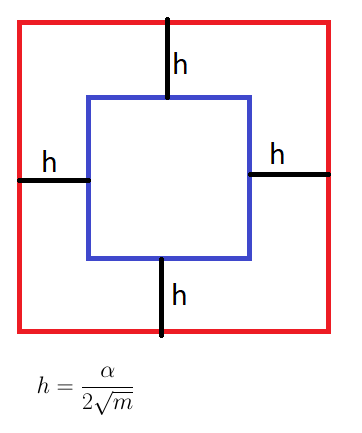
\includegraphics[scale=1]{Th21Pic1.png}

	$A \subset G \subset Int(Q_1)$

	$\sup_G f \leqslant \sup_{\overline{Q_1}} f < + \infty$

	При этом $\lambda G$ может быть выбрана сколь угодно близко к $\lambda A = 0$ по регулярности меры Лебега.

	\item $\lambda A > 0, \sup_A f < c$

	Возьмём $c_1$:

	$\sup_A f < c_1 < c$

	Выберем $\epsilon$ так чтобы

	$\epsilon \cdot c_1 < \lambda A \cdot (c - c_1) ~~~~ \textbf{(*)}$

	$G_{\epsilon}$ - такое множество, что $A \subset G_{\epsilon}, G_{\epsilon}-$открытое, $\lambda(G_{\epsilon} \setminus A) < \epsilon$

	$G_1 := f^{-1}((- \infty; c_1)) \cap G_{\epsilon} - $ открытое

	$\lambda(G_1 \setminus A) < \epsilon$

	$\lambda G_1 \cdot \sup_{G_1} f \leqslant (\lambda A + \epsilon) \cdot c_1 < \lambda A \cdot c$ (из $\textbf{(*)}$)

	(так как $G \subset f^{-1}(- \infty; c_1)$, то есть $f$ на $G_1$ не больше $c_1$)

	$\inf(\lambda G \cdot \sup_G f) < \lambda A \cdot c$

	Переходя к $\inf$ по $c$, получаем что требовалось
\end{enumerate}

\section{Теорема о преобразовании меры при диффеоморфизме}
$\Phi: O \subset \mathds{R}^m \rightarrow \mathds{R}^m$ - Диффеоморфизм, $\forall A \in \mathds{M}^m, A \subset O$

$\lambda(\Phi(A)) = \int_A |\det \Phi' (x)| d \lambda(x)$

\emph{Доказательство:}

Пусть $\nu A = \lambda(\Phi(A))$, проверим, что $|\det \Phi' (x)|$ - плотность $\nu$ относительно $\lambda$.

Обозначим $J(x) = |\det \Phi' (x)|$

Проверим $\forall A: \inf_{x \in A} J(x) \cdot \lambda A \leqslant \nu A \leqslant \sup_{x \in A} J(x) \cdot \lambda A$

Достаточно проверить только правую, так как левая эквивалентна $\lambda A \leqslant (\inf_{x \in A} J_{\Phi}(x))^{-1} \nu A$, а $(\inf_{x \in A} J_{\Phi}(x))^{-1} = \sup_{x \in A} (J_{\Phi}(x))^{-1} = \sup_{y \in A'} J_{\Phi^{-1}}(y)$ (где $A' = \Phi(A), A = \Phi^{-1}(A')$)

Тогда $\lambda(\Phi^{-1}(A')) \leqslant \sup_{y \in A'} J_{\Phi^{-1}}(y) \cdot \lambda A'$ экваивалентно правому неравенству, но для $\Phi^{-1}$

Докажем правую часть

\begin{enumerate}
	\item $A$ - кубическая ячейка, $A \subset \overline{A} \subset O$
	
	Пусть это неверно, тогда $\exists Q: \sup_{x \in Q} J(x) \cdot \lambda Q < \nu Q$. Возьмём $c:  \sup_{x \in Q} J(x) < c$, тогда $c \cdot \lambda Q < \nu Q$. Разобьём $Q$ на $2^m$ кубических ячеек, сторона каждой из которых в 2 раза меньше стороны исходной, тогда $\exists Q_1: c \cdot \lambda Q_1 < \nu Q_1$. Аналогично делим $Q_1$, по индукции строим вложенную последовательсность таких ячеек. $\forall n: c \cdot \lambda Q_n < \nu Q_n (*)$
	
	Рассмотрим $a = \bigcap Q_n$, при этом $J(a) = |def \Phi'(a)| < c$. Тогда по лемме $\exists B(a, \delta):$ при $Q_n \subset B(a, \delta): \lambda \Phi(Q_n) < c \cdot \lambda Q_n$ - противоречие с (*).
	
	\item $A$ - открытое множество. Тогда $A = \bigsqcup A_i$. (кубические ячейки). Способ разбиения был в прошлом семе.
	
	Тогда $\nu A = \sum \nu A_i \leqslant \sum \sup_{A_i} J \cdot  \lambda A_i \leqslant \sum \sup_{A} J \cdot \lambda A_i = \sup_{A} J \cdot \sum \lambda A_i = \sup_{A} J \cdot  \lambda A$ 
	
	\item $A$ - произвольное измеримое.
	
	$\nu A \leqslant \nu G$ ($A \subset G, G$ - открытое), тогда $\nu A \leqslant \sup_G J \cdot \lambda G \Rightarrow \nu A \leqslant \inf_{A \subset G - open set}(\sup_G J \cdot \lambda G) \Rightarrow \nu A \leqslant \sup_A J \cdot \lambda A$ (из леммы)
	
\end{enumerate}

\section{Теорема о гладкой замене переменной в интеграле Лебега}
$\Phi: O \subset \mathds{R}^m \rightarrow \mathds{R}^m$ - диффеоморфизм

$O' = \Phi(O)$~--- открытое

$f$ задана на $O', f \geqslant 0$, измерима по Лебегу, тогда

$\int_{O'}f(y) \cdot d \lambda(y) = \int_O f(\Phi(x)) \cdot |\det \Phi'(x)| \cdot d \lambda(x)$

\emph{Доказательство:}

Изи.

$\nu(A) = \lambda \Phi (A), \nu$ имеет плотность $J \Phi$ относително $\lambda$.

Применить теорему об интеграле по взвешенному образу меры.


%\section{Теорема Фубини}
%	$(X, \alpha, \mu)$ и $(Y, \beta, \nu)$ - пространства с мерами, причем $\mu , \nu$ --- $\sigma$-конечны\\
%	на $X \times Y$ есть $\alpha \otimes \beta$, причем $m(A \times B) = \mu A \cdot \nu B$ --- произведение мер --- $\sigma$-конечная мера на $\alpha \times \beta$\\
%	$(X \times Y), \alpha \otimes \beta, m$ --- произведение пр-в с мерой\\
%	Обозначение : $C \subset X \times Y, x \in X$ тогда $C_x = {y : (x, y) \in C}$ --- Сечение I рода\\
%	$C_y = {x : (x, y) \in C}$ --- Сечение II рода\\


\section{Теорема (принцип Кавальери)}
	$(X, \alpha, \mu)$ и $(Y, \beta, \nu)$~--- пространства с мерами, причем $\mu$, $\nu$~--- $\sigma$-конечные и полные\\
	$m = \mu \times \nu$, $C \in \alpha\otimes\beta$, тогда:\\
	\begin{enumerate}
		\item
		При п.в. $x$ $C_x$ измеримо ($\nu$-измеримо), т.е. $C_x \in \beta$
		\item
		Функция $x \rightarrow \nu C_x$~--- измеримая (в широком смысле) на $X$\\ \\
		NB: $\phi$~--- измерима в широком смысле, если она задана при п.в. x, и $\exists f : X \rightarrow R'$~--- измеримая и $\phi = f$ п.в. При этом $\int_X \phi = \int_X f$ (по опр.)
		\item
		$m C = \int_X \nu(C_x) \cdot d\mu(x)$
	\end{enumerate}
	\emph{Доказательство:}
		Рассмотрим $D$~--- совокупность все множеств $C$, для которых утверждение теоремы верно.\\
		$\rho = \alpha\times\beta$~--- полукольцо измеримых <<прямоугольников>>.\\
		\begin{enumerate}
			\item
				$\rho \subset D$\\
				$C = A \times B$. то есть $\forall x\ C_x = 
                    \begin{cases}
                        \emptyset, x \not\in A;\\
                        B, x \in A
                    \end{cases}$\\
				$x \rightarrow \nu(C_x)$, функция $\nu(B) \cdot \chi_A(x)$ --- изм.\\
				$\int_X \nu(C_x)d\mu = \nu B \int_X \chi_A(x)d\mu(x) = \nu B \cdot \mu A = m C$
			\item
				$E_i \in D$, $E_i$ дизъюнктны $\Rightarrow$ $E := \bigsqcup E_i \in D$\\
				при п.в. $x$ $(E_i)_x$~--- измеримы\\
				при п.в. $x$ все $(E_i)_x$~--- измеримы, $E_x = \bigsqcup (E_i)_x$~--- измеримо.\\
				$\nu E_x = \sum \nu (E_i)_x$ ($\nu (E_i)_x$ --- изм. как функция от $x$) $\Rightarrow$ функция $ x \rightarrow \nu E_x$ --- измерима\\
				$\int_X \nu E_x d\mu(x) = \sum_{i}\int\nu(E_i)_x d\mu(x) = \sum_{i}m E_i = m E$
			\item
				$E_i \in D$, $E_1 \supset E_2 \supset \ldots ; m E_i < +\infty$. Тогда $E := \bigcap E_i \in D$\\
				$\int_X\nu(E_i)_x d\mu = m E_i < +\infty\ (*)$\\
				функция $x \rightarrow \nu(E_i)_x$ --- суммируема $\Rightarrow$ п.в. конечна.\\
				при всех $x$ $(E_i)_x \downarrow E_x$, т.е. $(E_1)_x \supset (E_2)_x \supset \ldots $ и $\bigcap(E_i)_x = E_x$\\
				при п.в. $x$ $\nu(E_i)_X$~--- конечны (для таких $x$).\\
				Тогда $E_x$ --- измерима и $\lim \nu(E_i)_x = \nu E_x$ по непр-ти меры $\nu$ сверху.\\
				(Th. Лебега) $|\nu(E_i)_x| \leq \nu(E_1)_x$ --- сумм. $\Rightarrow$ функция $x \rightarrow \nu E_x$ --- изм.\\
				$\int_X\nu E_x d\mu = \lim\int_X\nu(E_i)_x d\mu = \lim m E_i = m E$ (нерп. сверху меры $m$). Этот предельный переход корректен как раз по теореме Лебега ($f_n \rightarrow f$ п.в. $g$ : $|f_n| \leq g$ --- сумм. Тогда $\int f_n \rightarrow \int f$).\\
				NB: мы доказали про пересечения и про объединения (пусть пересечения убывающие, а объединения --- дизъюнктные, но это лечится). Поэтому $\cap_j(\cup_i A_{i, j}) \in D$, если $A_{i,j} \in \rho$ ($\rho \subset D$).
				
			\textcolor{red}{Я точно не уверен, но вроде, дальше написан бред}
			\item
				$m E = 0 \Rightarrow E \in D$\\
				$\exists H \in D, H$ имеет вид $\cap(\cup A_{i, j})$, где все $A_{i,j} \in \rho$ \\
				$E \subset H , m H = 0$ из п.5 т. о продолжении \textcolor{red}{ЧТО?! поясните плез}\\
				$0 = m H = \int_X\nu H_x d\mu(x) \Rightarrow \nu H_x ~ 0$ ($ = 0$ при п.в. $x$).\\
				$E_x \subset H_x \Rightarrow E_x$ --- $\nu$-изм. (из полноты $\nu$) и $\nu E_x = 0$ п.в. $x$\\
				$\int_X \nu E_x d\mu = 0 = m E$
			\item
				\textcolor{red}{Неизмерима, но мера меньше $\infty$? ШТА?}
				$C$ --- неизм, $m C < +\infty$. Тогда $C \in D$.\\
				$C = H \setminus e$, где $m e = 0$, H --- вида $\cap(\cup A_{i, j})$.\\
				$C_x = H_x \setminus e_x$ --- изм. при п.в. $x$\\
				$\nu e_x = 0$ п.в.$x$ (проверено в п.4)\\
				$\nu C_x = \nu H_x = \nu e_x$ --- изм. п.в.$x$\\
				$\int_X\nu C_x = \int_X\nu H_x - \int_X\nu e_x = \int\nu H_x = m H = m C$.
			\item
				\textcolor{red}{Что тут вообще написано? Что такое $\subset \cap(X_k \times Y_n)$}
				$C$ --- $m$-изм. произвольное\\
				$X = \sqcup X_k, Y = \sqcup Y_n$ ($\mu X_k$ --- кон, $\nu Y_n$ --- кон.).\\
				$C = \sqcup_{k,n}(\subset \cap(X_k \times Y_n)) \in D$ (по п.2) (т.к. $\subset \cap(X_k \times Y_n) \in D$ по п.5)
		\end{enumerate}


\section{Теорема Тонелли}
$<\mathds{X}, \alpha, \mu>$, $<\mathds{Y}, \beta, \nu>$ - пространства с мерой\\
$\mu$, $\nu$ - $\sigma$-конечны, полные \\
$m = \mu \times \nu$ \\
$f: \mathds{X} \times \mathds{Y} \rightarrow \overline{R}$, $f \geq 0$, f - измерима относительно m \\
\emph{Тогда:}
\begin{enumerate}
	\item при \textit{почти всех} $x \in X$ $f_x$ - измерима на $\mathds{Y}$, \\
	 где $f_x : \mathds{Y} \rightarrow \overline{R}$, $f_x(y) = f(x, y)$ \\
	 (симметричное утверждение верно для y)
	 \item Функция $x \mapsto \phi(x) = \int\limits_{\mathds{Y}}f_x d\nu = \int\limits_{\mathds{Y}}f(x, y) d\nu(y) $ - $\text{измерима}^{\text{*}}$ на $\mathds{X}$ \\
	 (симметричное утверждение верно для y)
	 \item $\int\limits_{\mathds{X} \times \mathds{Y}}f(x, y)dm = \int\limits_{\mathds{X}}\phi(x)d\mu = \int\limits_{\mathds{X}}(\int\limits_{\mathds{Y}} f(x, y)d\nu(y))d\mu(x) = \int\limits_{\mathds{Y}}(\int\limits_{\mathds{X}}f(x,y)d\mu(x))d\nu(y)$
\end{enumerate}
\emph{Доказательство:} \\
Докажем в 3 пункта, постепенно ослабляя ограничения на функцию f
\begin{enumerate}
	\item Пусть $C \subset \mathds{X} \times \mathds{Y}$ - измеримо относительно m, $f = \chi_C$
	\begin{enumerate}
		\item $f_x(y) = \chi_{C_x}(y)$, где $C_x$ - сечение по x \\
		$C_x$ - измеримо при \textit{почти всех} x, так как это одномерное сечение, таким образом $f_x$ - измеримо, при \textit{почти всех} x.
		\item $\phi(x) = \int\limits_{\mathds{Y}}f_xd\nu = \nu C_x$ - по принципу Кавальери это $\text{измеримая}^{\text{*}}$ функция.
		\item $\int\limits_{\mathds{X}}\phi(x)d\mu = \int\limits_{\mathds{X}}\nu C_x d \mu \overset{\text{Кавальери}}{=} mc \overset{\text{опр.инт}}{=} \int\limits_{\mathds{X} \times \mathds{Y}}\chi_C dm = \int\limits_{\mathds{X} \times \mathds{Y}}f(x, y) dm$
	\end{enumerate}
	\item Пусть f - ступенчатая, $f \geq 0$, $f = \sum\limits_{\text{кон}}a_k \chi_{C_k}$ \\
	\begin{enumerate}
		\item $f_x = \sum a_k \chi_{(C_k)_x}$ - измерима при почти всех x \\
		\item $\phi(x) = \sum a_k \nu(C_k)_x$ - $\text{измерима}^{\text{*}}$ как конечная сумма 	измеримых\\
		\item $\int\limits_{\mathds{X}}\phi(x) = \int\limits_{\mathds{X}}\sum\limits_{\text{кон}}a_k \nu (C_k)_x d \mu =
		\sum\limits_{\text{кон}}\int\limits_{\mathds{X}}a_k \nu (C_k)_x d \mu =
		\sum a_k m C_k = \int\limits_{\mathds{X} \times \mathds{Y}}f dm$
	\end{enumerate}
	\item Пусть f - измеримая, $f \geq 0$ \\
	$f = \lim\limits_{n \rightarrow +\infty}g_n$, где $g_n \geq 0$ - ступенчатая, $g_n$ - монотонно возрастает к f (из Теоремы об апроксимации измеримой функции ступенчатыми)
	\begin{enumerate}
		\item $f_x = \lim\limits_{n \rightarrow +\infty}(g_n)_x \Rightarrow f_x$ - измерима при \textit{почти всех} x.
		\item $\phi(x) = \int\limits_{\mathds{Y}}f_xd\nu \overset{\text{т.Леви}}{=} \lim \int\limits_{\mathds{Y}}(g_n)_xd\nu$ \\
		$\phi_n(x) := \int\limits_{\mathds{Y}}(g_n)_xd\nu$ - измерима по пункту 1 \\
		$0 \leq (g_n)_x - \text{возрастает}$, тогда $\phi(x)$ - измерима, $\phi_n(x) \leq \phi_{n+1}(x) \leq ...$ и $\phi_n(x) \rightarrow \phi(x)$
		\item $\int\limits_{\mathds{X}}\phi(x)d\mu \overset{\text{т.Леви}}{=} \lim\limits_{n \rightarrow +\infty}\int\phi_n(x)d\mu \overset{\text{п.2}}{=}\lim\limits_{n \rightarrow +\infty}\int\limits_{\mathds{X} \times \mathds{Y}}g_ndm \overset{\text{т.Леви}}{=} \int fdm$
	\end{enumerate}
\end{enumerate}

\section{Формула для Бета-функции}
$B(s, t) = \int\limits_{0}^{1}x^{s-1}(1-x)^{t-1}$, где s и t > 0 - Бета-функция \\
$\Gamma(s) = \int\limits_{0}^{+\infty}x^{s-1}e^{-x}dx$, где s > 0, тогда $B(s, t) = \frac{\Gamma(s)\Gamma(t)}{\Gamma(s+t)}$ \\
\emph{Доказательство:}\\
$\Gamma(s)\Gamma(t) = \int\limits_{0}^{+\infty}x^{s-1}e^{-x}(\int\limits_{0}^{+\infty}y^{t-1}e^{-y}dy)dx =
\begin{bmatrix}y \rightarrow u \\ y = u - x \end{bmatrix} =
\int\limits_{0}^{+\infty}x^{s-1}(\int\limits_{x}^{+\infty}(u-x)^{t-1}e^{-u}du)dx=\\
= \int\limits_{\begin{matrix}x \geq 0 \\ u \geq x \end{matrix}}...=$ меняем порядок интегрирования\\
$= \int\limits_{0}^{+\infty}du\int\limits_{0}^{u}dx (x^{s-1}(u-x)^{t-1}e^{-u})
= \begin{bmatrix} x \rightarrow v\\ x = uv \end{bmatrix}
= \int\limits_{0}^{+\infty}e^{-u}(\int\limits_{0}^{1}u^{s-1}v^{s-t}u^{t-1}(1-v)^{t-1}udv)du =\\
= \int\limits_{0}^{+\infty}u^{s+t-1}e^{-u}(\int\limits_{0}^{1}v^{s-1}(1-v)^{t-1}dv)du = B(s,t)\Gamma(s+t)$, чтд.
\section{Объем шара в $\mathbb R^m$}
$B(0, R) \subset \mathbb{R}^m$ \\
$\lambda_m(B(0, R)) = \int\limits_{B(0, R)}1d\lambda_m = \int \mathcal{J} = \\
= \int\limits_{0}^{R}dr\int\limits_{0}^{\pi}d\phi_1\dots\int\limits_{0}^{\pi}d\phi_{m-2} \int\limits_{0}^{2\pi}d\phi_{m-1} \cdot r^{m-1}(\sin\phi_1)^{m-2} \dots (\sin\phi_{m-2}) =\rightarrow\\
\int\limits_{0}^{\pi}(\sin\phi_k)^{m-2-(k+1)} = B({\frac{m-k}{2}}; \frac{1}{2}) = \frac{\Gamma(\frac{m-k}{2})\Gamma(\frac{1}{2})}{\Gamma(\frac{m-k}{2}+\frac{1}{2})} $\textcolor{red}{почему так? надо бы поподробней расписать}$\\
\rightarrow= \frac{R^m}{m} \frac{\Gamma(\frac{m-1}{2}) \Gamma(\frac{1}{2})}{\Gamma(\frac{m}{2})} \frac{\Gamma(\frac{m-2}{2})\Gamma(\frac{1}{2})}{\Gamma(\frac{m-1}{2})} \cdots \frac{\Gamma(1) \Gamma(\frac{1}{2})}{\Gamma(\frac{3}{2})} 2\pi =\\
= \frac{\pi R^m}{\frac{m}{2}} \frac{\Gamma(\frac{1}{2})^{m-2}}{\Gamma(\frac{m}{2})} = \frac{\pi^{\frac{m}{2}}}{\Gamma(\frac{m}{2}+1)}R^m$

\section{Теорема о вложении пространств $L^p$}

$ \mu E < +\infty$, $1 \leq s < r \leq + \infty$

\textbf{\emph{Тогда:}}

\begin{enumerate}
	\item $ L_r(E, \mu)  \subset \L_s(E, \mu)$
	\item $ \forall f$~--- измеримая $: ||f||_s \leq \mu E^{1/s - 1/r} ||f||_r$
\end{enumerate}

\textbf{\emph{Доказательство:}}

\begin{itemize}
	\item $2 \Rightarrow 1$ (Это очевидно: достаточно рассмотреть неравенство из пункта 2. Из него следует, что $ ||f||_s \leq const \cdot ||f||_r $. см. опред. $ L_p $)

	\item Рассмотрим два случая:
	\begin{enumerate}
		\item $ r = + \infty $ (очев.)
		$$ ||f||_s = (\int |f|^s \cdot 1)^{1/s} \leq ((esssup|f|)^s \int 1 d\mu)^{1/s} = ||f||_{\infty} \cdot \mu E^{1/s} $$ (последнее по определению $ esssup $)

		\item $ r < + \infty $

		$$ (||f||_s)^{s} = \int |f|^s \cdot 1 d\mu  \leq
		(\int |f|^r)^\frac{s}{r} \cdot (\int 1^\frac{r}{r - s})^\frac{r - s}{r} =
		(||f||_r)^s \cdot \mu E^{1 - \frac{s}{r}} $$ (существенный шаг: применить неравество Гельдера)
	\end{enumerate}
\end{itemize}

\section{Теорема о сходимости в $L_p$ и по мере}
$ 1 \leq p < +\infty $

$ f_n \in L_p(\mathbb{X}, \mu)$

\begin{enumerate}


	\item \begin{itemize}
		\item $ f \in L_p $
		\item $ f_n \rightarrow f $ в $ L_p $
	\end{itemize}
	\textbf{Тогда:} $ f_n \stackrel{\mu}{\Rightarrow} f $ (по мере)

	\item \begin{itemize}
		\item $ f_n \stackrel{\mu}{\Rightarrow} f $ (либо если $ f_n \rightarrow f $  почти везде)
		\item $ |f_n| \leq g $ почти везде при всех $n$; $g \in L_p$
	\end{itemize}
	\textbf{Тогда:} $ f_n \rightarrow f $ в $ L_p $
\end{enumerate}

\textbf{\emph{Доказательство:}}

\begin{enumerate}
	\item $$ X_n(\epsilon) := X(|f_n - f| \geq \epsilon) $$

	$$ \mu X_n(\epsilon) \overset{\text{т.к.}\ \frac{|f_n-f|}{\epsilon} \geq 1}{\leqslant} \int\limits_{X_n} (\frac{|f_n - f|}{\epsilon})^p  =
	\frac{1}{\epsilon^p} \int\limits_{X_n} |f_n - f|^p \leq
	\frac{1}{\epsilon^p} \int\limits_{X} |f_n - f|^p = $$
	$$ = \frac{1}{\epsilon^p} (||f_n - f||_p)^p \stackrel{n \rightarrow \infty}{\rightarrow} 0$$

	\item $ f_n \stackrel{\mu}{\Rightarrow} f $ Тогда $ \exists n_k \mid f_{n_k} \rightarrow f $ почти везде.

	Тогда $ |f| \leq g $ п. в.

	$ |f_n - f|^p \leq (2g)^p $ -- сумм. функции т. к. $ g \in L_p $

	$ (||f_n - f||_p)^p = \int\limits_{X} |f_n - f|^p d\mu \stackrel{n \rightarrow \infty}{\rightarrow} 0 $ (по теореме Лебега)

\end{enumerate}

\section{Полнота $L^p$}
$ L_p(E, \mu) ~ ~ 1 \leq p < \infty $ -- полное

То есть любая фундаментальная последовательность сходиться по норме $ ||f||_p $.

$$(\forall \epsilon > 0 ~ \exists N ~ \forall n, k ~ ||f_n - f_k||_p < \epsilon) \Rightarrow (\exists f : ||f_n - f||_p \rightarrow 0)$$


\textbf{\emph{Доказательство:}}

\begin{enumerate}
	\item Построим $ f $.

	Рассмотрим фундаментальную последовательность $ f_n $.

	$ \exists N_1 $ при $ n_1, k > N_1 ~ ||f_{n_1} - f_k|| < \frac{1}{2}$

	$ \exists N_2 $ при $ n_2, k > N_2, N_1 ~ ||f_{n_2} - f_k|| < \frac{1}{4}$

	\dots

	Тогда: $ \sum_{k = 1}^{\infty} || f_{n_{k+1}} - f_{n_k} || < 1$

	$ f = \lim\limits_{k \rightarrow \infty} f_{n_k}$

	Докажем, это функция $ f $ корректно задана:
	\begin{itemize}
		\item
		$ S_N (x) := \sum_{k = 1}^{N}|f_{n_{k+1}} - f_{n_k}|$

		$ ||S_N||_p \leq \sum_{k = 1}^{N} || f_{n_{k+1}} - f_{n_k} || < 1$

		Тогда по Теореме Фату: $ ||S||_p \leq 1 $

		Тогда $ |S|^p $ -- суммируема

		Тогда $ S(x) $ конечна при п. в. $ x $  и ряд $ \sum f_{n_{k + 1}} - f_{n_k} $ абс. сходитс, а значит и просто сходится при п. в. $ x $

		$ f:= f_{n_1} +  \sum f_{n_{k + 1}} - f_{n_k} $ т. е. $ f = $ п. в. $ \lim\limits_{k \rightarrow \infty} f_{n_k} $
	\end{itemize}

	\item Проверим, что $ f_n \rightarrow f $ в $ L_p $

	Т. к. $ f_n $ -- фунд., то $ \forall \epsilon > 0 ~ \exists N ~ \forall n, n_k > N ~ ~ ||f_n - f_{n_k} || < \epsilon \Rightarrow
	|| f_n  - f_{n_k} ||^p  = \int\limits_{E} |f_n  - f_{n_k}|^p d\mu < \epsilon^p $

	Тогда по теореме Фату: $ \int\limits_{E} |f - f_n|^p \leq \epsilon^p$

	Тогда $ \forall \epsilon > 0 ~ \exists N ~ \forall n > N ~ || f - f_n ||_p < \epsilon $


\end{enumerate}

\textbf{\emph{Замечание:}} $ L_{\infty} $ -- полное (упражнение)

\section{Лемма Урысона}
$X$~--- нормальное топологическое пространство, то есть:
\begin{enumerate}
    \item Все одноточечные множества замкнуты.
    \item Любые два непересекающихся замкнутых множества отделимы окрестностями:\\
    $A,B$~--- замкнуты, $A \cap B = \emptyset$ $\Rightarrow$ $\exists A_1,B_1$~--- открыты, $A_1 \cap B_1 = \emptyset$,
    $A \subset A_1$, $B \subset B_1$.
\end{enumerate}

$F_0$, $F_1$~--- замкнуты, $F_0 \cap F_1 = \emptyset$.

\emph{Тогда:} $\exists f: X \rightarrow [0,1]$, непрерывная (в смысле топологического определения непрерывности), равная $0$ на $F_0$ и равная $1$ на $F_1$.
\\\\
\emph{Доказательство}:
\textcolor{red}{TODO!}

\section{Плотность в $L^p$ непрерывных финитных функций}
$(\mathbb{R}^m, \mathbb{A}, \lambda_m)$\\

$E \subset \mathbb{R}^m -$ изм. Тогда множество финитных непрерывных функций плотно в $L_p(E, \lambda_m), p \in [1; +\infty]$\\

\emph{Доказательство}:

\begin{enumerate}
	\item  Раскроем определение плотности: $\forall f \in L_p(E, \mu) \ \forall \epsilon > 0 \ \exists \varphi \in C_0(\mathbb{R}^m): ||f - \varphi|_E ||_p < \epsilon$. Таким образом достаточно научиться приближать $f$ и  $\varphi$ ступенчатыми функциями $f_n$: $||f-f_n||_p < \epsilon /2 $ и $||\varphi-f_n||_p < \epsilon /2 $

	\item	 \textcolor{red}{TODO!}

\end{enumerate}


\section{Теорема о непрерывности сдвига}
\emph{Обозначения}:

$f_h := f(x+h)$ \\
$[0, T] \subset \mathbb{R}$. Будем считать, что $L_p[0, T]$ состоит из $T$-периодических функций $\mathbb{R} \rightarrow \overline {\mathbb{R}}$. Отсюда $\int_{0}^{T} f = \int_{a}^{a+T} f.$ \\
$\widetilde{C}[0, T] = {f \in C[0, T]: f(0) = f(T) }. ||f|| = max_{x\in[0,T]}|f(x)|$ \\
NB: $f \in \widetilde{C}[0, T] \Rightarrow f$ равномерно непрерывна (по т. Кантора).

\emph{Формулировка}:
\begin{enumerate}
	\item $f - $ рвнм. непр. на $\mathbb{R}^m$. Тогда $||f-f_h||_\infty \rightarrow 0$ при $h\rightarrow 0$.
	\item $1 \leq p < + \infty \ f \in L_p(\mathbb{R}^m, \lambda_m)$. Тогда $||f-f_h||_p \rightarrow 0$.
	\item $f \in \widetilde{C}[0, T]$. Тогда $||f-f_h||_\infty \rightarrow 0$.
	\item $1 \leq p < + \infty \  f \in L_p[0; T]$. Тогда $||f-f_h||_p \rightarrow 0$.
\end{enumerate}

\emph{Доказательство}:

\begin{enumerate}
	\item 1 и 3 свойства следуют из определения рвнм. непр-ти:
		$\forall \epsilon > 0 \ \exists \delta > 0 \  \forall x \in \mathbb{R}^m \ \forall h: |h| < \delta$ верно, что $|f(x) - f(x+h)| < \epsilon$, то есть $||f-f_h||_\infty < \epsilon$
		(это для св-ва 1, во втором случае $x$ из $[0,T]$).
	\item \textcolor{red}{TODO!}
\end{enumerate}

\section{Теорема об интеграле с функцией распределения}
\textcolor{red}{Проверить формулировку, тут, вроде, какая-то херня написана}

\textcolor{red}{чё за измеримость по Борелю???}

$(\mathbb{R}, B, X)$ \\
$f:\mathbb{R}\rightarrow\mathbb{R}, f \ge 0,$ изм. по Борелю, п.в. конечн.\\
$h: X \rightarrow \overline{\mathbb{R}}$ с функцией распределения $H(t)$\\

$\mu_H$ -- мера Бореля-Стилтьеса (мера Лебега-Стилтьеса на $B$)\\

\emph{Тогда} $\int\limits_X f(h(x))d\mu(x) = \int\limits_{\mathbb{R}}f(t)d\mu_{H}(t)$

\emph{Доказательство}:
Следует из теоремы о вычислении интеграла по взвешенному образу меры, положив $<Y, C, \nu> = <\mathbb{R}, B(\mathbb{R}), h(\mu)>, \Phi = h, \omega = 1$

\section{Теорема о свойствах сходимости в гильбертовом пространстве}
\begin{enumerate}
	\item $x_n \rightarrow x, y_n \rightarrow y \Rightarrow \langle x_n, y_n \rangle \rightarrow \langle x, y \rangle$

	\item $\sum x_k$ сходится, тогда $\forall y: \sum \langle x_k, y \rangle = \langle \sum x_k, y \rangle$

	\item $\sum x_k$ - ортогональный ряд, тогда $\sum x_k$ - сх $\Leftrightarrow \sum |x_k|^2$ сходится, при этом $|\sum x_k|^2 = \sum |x_k|^2$

\end{enumerate}

\emph{Доказательство}

\begin{enumerate}
	\item $|\langle x_k, y_k \rangle - \langle x, y \rangle| = |\langle x_k, y_k \rangle - \langle x_k, y\rangle  + \langle x_k, y\rangle  - \langle x, y\rangle | \leqslant |\langle x_k, y_k - y\rangle | + |\langle x_k - x, y\rangle | \leqslant |x_k| \cdot |y_k - y| + |x_k - x| \cdot |y| \rightarrow 0$ (так как огр $\cdot$ б.м. +  б.м. $\cdot$ огр $\rightarrow$ 0)

	\item $S_n = \sum\limits_{k = 1}^{n} x_k$

	$\langle \sum\limits_{k = 1}^n x_k, y\rangle  = \sum\limits_{k = 1}^n \langle x_k, y\rangle $

	Устремляя $n$ к $\infty$, получаем требуемое равенство

	\item Обозначим $C_n := \sum\limits_{k = 1}^n |x_k|^2$

	 $|S_n|^2 = \langle \sum\limits_{k = 1}^n x_k, \sum\limits_{j = 1}^n x_j\rangle  = \sum\limits_{k, j}^n \langle x_k, x_j\rangle  = \sum\limits_{k = 1}^n \langle x_k, x_k\rangle $ (так как $k \neq j \Rightarrow \langle x_k, x_j\rangle  = 0$) $= \sum\limits_{k = 1}^n |x_k|^2 = C_n$

	 Аналогично, $||S_n|^2 - |S_m|^2| = |C_n - C_m|$

	 Тогда $C_n, |S_n|^2$ фунадментальны одновременно $\Rightarrow$ сходятся одновременно при устремлении $n$ к $\infty$
\end{enumerate}

\section{Теорема о коэффициентах разложения по ортогональной системе}

$\{e_k\}$ {{---}} ортогональная система в $\mathds{H},\ x \in \mathds{H}, x = \sum\limits_{k=1}^{+\infty} c_k \cdot e_k$

\emph{Тогда:}
\begin{enumerate}

	\item $\{e_k\}$ {{---}} Л.Н.З.

	\item $c_k = \dfrac{\langle x, e_k \rangle}{||e_k||^2}$

	\item $c_k \cdot e_k$ {{---}} проекция $x$ на прямую $\{te_k \mid t \in \mathbb{R}\ (\text{или}\ \mathbb{C})\}$\\
	Иными словами, $x = c_k \cdot e_k + z$, где $z \bot e_k$

\end{enumerate}

\emph{Доказательство:}

\begin{enumerate}

	\item Пусть $\sum\limits_{k=1}^{N} \alpha_k e_k = 0$. Умножим скалярно на $e_m\ (1 \leqslant m \leqslant N)$\\ \\
	Получим: $\alpha_m ||e_m||^2 = 0 \Rightarrow \alpha_m = 0 \Rightarrow$ комб. тривиальная $\Rightarrow$ Л.Н.З.

	\item $\langle x, e_m \rangle = \sum\limits_{k=1}^{+\infty} \langle c_k e_k, e_m \rangle = c_m \cdot ||e_m||^2$ (верно в силу сходимости ряда)

	\item $x = c_k \cdot e_k + z$. Доказать: $z \bot e_k$.\\
	$\langle z, e_k \rangle = \langle x - c_k e_k, e_k \rangle = c_k \cdot ||e_k||^2 - c_k\cdot ||e_k||^2 = 0$

\end{enumerate}

\section{Теорема о свойствах частичных сумм ряда Фурье. Неравенство Бесселя}

$\{e_k\}$ {{---}} ортогональная система в $\mathds{H},\ x \in \mathds{H}, n \in \mathbb{N}$

$S_n = \sum\limits_{k=1}^{n} c_k(x)e_k,\ \pazocal{L} = Lin(e_1, e_2, \ldots e_n) \subset \mathds{H}$

\emph{Тогда:}

\begin{enumerate}

	\item $S_n$ {{---}} орт. проекция $x$ на пр-во $\pazocal{L}$. Иными словами $x = S_n + z,\ z \bot \pazocal{L}$

	\item $S_n$ {{---}} наилучшее приближение $x$ в $\pazocal{L}\ (||x - S_n|| = \min\limits_{y \in \pazocal{L}} ||x - y||)$

	\item $||S_n|| \leqslant ||x||$

\end{enumerate}

\emph{Доказательство:}

\begin{enumerate}

	\item
	\begin{enumerate}
		\item $z = x - S_n$

		\item $z \bot \pazocal{L} \Leftrightarrow \forall k = 1, 2 ...n : z \bot e_k$

		\item $\langle z, e_k \rangle = \langle x, e_k \rangle - \langle S_n, e_k \rangle = c_k ||e_k||^2 - c_k ||e_k||^2 = 0$
	\end{enumerate}

	\item $||x - y||^2 = ||S_n + z - y||^2 = ||(S_n - y) + z||^2 = ||S_n - y||^2 + ||z||^2 \geqslant$ $\geqslant ||z||^2 = ||x - S_n||^2$

	\item $||x||^2 = ||S_n||^2 + ||z||^2$ (теорема о сумме орт. ряда) $\geqslant ||S_n||^2$
\end{enumerate}

\emph{Cледствие:} Неравенство Бесселя\\

$\forall \{e_k\}$ {{--}} О.С. $:\sum\limits_{k=1}^{+\infty} |c_k(x)|^2 \cdot ||e_k||^2 \leqslant ||x||^2$

\section{Теорема Рисса -- Фишера о сумме ряда Фурье. Равенство Парсеваля}
$\{e_k\}$ -- орт. сист. в $\mathds{H}$, $x \in \mathds{H}$\\

\emph{Тогда}:
\begin{enumerate}
	\item Ряд Фурье $\sum\limits_{k=1}^{+\infty} c_k(x) e_k$ сходится в $\mathds{H}$
	\item $x =\sum\limits_{k=1}^{+\infty} c_k e_k + z \Rightarrow \forall k \ z \bot e_k$
	\item $x =\sum\limits_{k=1}^{+\infty} c_k e_k \Leftrightarrow \sum\limits_{k=1}^{+\infty} \vert c_k \vert^2 \|e_k\|^2=\|x\|^2$
\end{enumerate}

\emph{Доказательство:}
\begin{enumerate}
	\item
	Ряд Фурье -- ортогональный ряд\\
	его сходимость $\Leftrightarrow$ сходимости $\sum\limits_{k=1}^{+\infty} \vert c_k \vert^2 \|e_k\|^2$\\
	$\sum\limits_{k=1}^{+\infty} \vert c_k \vert^2 \|e_k\|^2 \le \|x\|^2$ по неравенству Бесселя
	\item
	$\langle z, e_k \rangle = \langle x - \sum c_i e_i, e_k \rangle = \langle x, e_k \rangle - \sum\limits_{i = 1}^{+\infty}  \langle c_i(x) e_i ,e_k \rangle = 0$
	\item
	$\Rightarrow$ - утв. 3 теоремы о св-вах сх-ти в гильбертовом пр-ве\\
	$\Leftarrow$
		Из п. 2 ряд ортог.\\
		$\|x\|^2=\|\sum c_k e_k\|^2 + \|z\|^2 = \sum \vert c_k \vert^2 \|e_k\|^2 + \|z\|^2 = \|x\|^2 + \|z\|^2 \Rightarrow z = 0$
\end{enumerate}

\iffalse
$\mathbf{TODO}$ Замечания. Не уверен, нужны ли они
\fi

\section{Теорема о характеристике базиса}

$\{e_k\}$~--- ортогональная система в $\mathds{H}$\\

\emph{Тогда} эквивалентны следующие утверждения:
\begin{enumerate}
	\item $\{e_1\}$~--- базис.
	\item $\forall x, y \in \mathds{H} \quad \langle x, y \rangle = \sum c_k(x)\overline{c_k(y)}\|e_k\|^2$ (обобщенное уравнение замкнутости)
	\item $\{e_k\}$~--- замкнутая система.
	\item $\{e_k\}$~--- полная система.
	\item $Lin(e_1, e_2, \mathellipsis)$~--- плотна в $\mathds{H}$
\end{enumerate}

\emph{Доказательство:}

\subsection{\texorpdfstring{$1 \Rightarrow 2$}{TEXT}}
$x=\sum c_k(x) e_k$ -- единственно (из геом. соображений: $c_k e_k$ -- проекция)\\
$\langle e_k, y \rangle = \overline{\langle y, e_k \rangle} = \overline{c_k(y)}\|e_k\|^2$\\
$\langle x, y \rangle = \sum c_k(x) \langle e_k, y \rangle = \sum c_k(x)\overline{c_k(y)}\|e_k\|^2$

\subsection{\texorpdfstring{$2 \Rightarrow 3$}{TEXT}}
$y:=x$\\
$\|x\|^2=\sum \vert c_k(x) \vert ^2 \|e_k\|^2$ (см. п. 3 из опр.)

\subsection{\texorpdfstring{$3 \Rightarrow 4$}{TEXT}}
Пусть $\forall k \quad x_0 \bot e_k$\\
$c_k(x_0)=\frac{\langle x_0, e_k \rangle}{\|e_k\|^2}=0$\\
$\|x_0\|^2=\sum \vert c_k(x_0) \vert^2 \|e_k\|^2 = 0$ (см. п. 2 из опр.)

\subsection{\texorpdfstring{$4 \Rightarrow 1$}{TEXT}}
$x =\sum\limits_{k=1}^{+\infty} c_k e_k + z \Rightarrow(\text{т. Рисса-Фишера (2)}) \  \forall k \ z \bot e_k \Rightarrow(\text{из полноты}) \ z = 0$ (см. п. 1 из опр.)

\subsection{\texorpdfstring{$4 \Rightarrow 5$}{TEXT}}
Пусть $Cl Lin(e_1, e_2, \mathellipsis) \ne \mathds{H}$, $x \in \mathds{H} \setminus Cl Lin(e_1, e_2, \mathellipsis)$\\
из т. Рисса-Фишера (2): $x =\sum\limits_{k=1}^{+\infty} c_k e_k + z \Rightarrow \forall k \ z \bot e_k \Rightarrow x =\sum\limits_{k=1}^{+\infty} c_k e_k \Rightarrow x \in Cl Lin(e_1, e_2, \mathellipsis)$\\
Противоречие.

\subsection{\texorpdfstring{$5 \Rightarrow 4$}{TEXT}}
$\forall k \ x_0 \bot e_k \Rightarrow x_0 \bot Lin(e_1, e_2, \mathellipsis) \Rightarrow x_0 \bot Cl Lin(e_1, e_2, \mathellipsis)( = \mathds{H}) \Rightarrow x_0 \bot x_0 \Rightarrow \|x_0\|^2 = 0 \Rightarrow x_0 = 0$

\section{Лемма о вычислении коэффициентов тригонометрического ряда}

Пусть $S_n \rightarrow f$ в $L_1(-\pi, \pi]$\\

\emph{Тогда}:

$a_k = \frac{1}{\pi}\int\limits_{-\pi}^{\pi}f(x)\cos kx\ dx \quad k = 0, 1, 2, \mathellipsis$

$b_k = \frac{1}{\pi}\int\limits_{-\pi}^{\pi}f(x)\sin kx\ dx \quad k = 0, 1, 2, \mathellipsis$

$c_k = \frac{1}{2\pi}\int\limits_{-\pi}^{\pi}f(x)e^{-ikx}\ dx \quad k = 0, 1, 2, \mathellipsis$


\emph{Доказательство:}

\textcolor{red}{Почему нельзя сказать, что коэффициенты~--- это коэффициенты ряда Фурье, а потому вычисляются как скалярные произведения???}

$S_n=\frac{a_0}2 + \sum\limits_{j=1}^n a_j \cos jx + b_j \sin jx$ (-- это $T_n$)

При $n \ge k:$

\begin{enumerate}
	\item
		$\int\limits_{-\pi}^{\pi} S_n(x) \cos kx dx = \int\limits_{-\pi}^{\pi} a_k \cos^2 kx dx = \pi a_k$
		(в силу ортогональности триг системы)
	\item
		$\vert \int\limits_{-\pi}^{\pi} S_n(x) \cos kx dx - \int\limits_{-\pi}^{\pi} f(x) \cos kx dx \vert \le \int\limits_{-\pi}^{\pi} \vert S_n(x)-f(X) \vert \cdot \vert \cos kx \vert \le \int\limits_{-\pi}^{\pi} \vert S_n(x) - f(x) \vert \rightarrow 0$
\end{enumerate}

Из 1 и 2 следует равенство для $a_k$. Аналогично доказывается и для других.

\section{Теорема Римана--Лебега}
$E \subset \mathds{R}^1$ -- измеримо\\ $f \in L_1(E, \lambda), ~ \lambda \text{- мера Лебега}$ \\
\emph{Тогда:} $$\int\limits_{E}f(x)e^{ikx}dx \xrightarrow[k \to +\infty]{} 0$$ и $$\int\limits_{E}f(x)cos(kx)dx \xrightarrow[k \to +\infty]{} 0$$
\emph{Доказательство:} \\
Пусть $f \equiv 0$ вне $E$, тогда можно считать, что $f \in L^1(\mathds{R}^1)$

Обозначим $e(x) = cos(x)$, или $sin(x)$, или $e^{ix}$, в зависимости от ситуации. Заметим, что $e(t + \pi) = -e(t)$

$\int\limits_{\mathds{R}}f(t)e(kt)  {\overset{t=\tau + \frac{\pi}{k}}{=}} \int\limits_{\mathds{R}}f(\tau + \frac{\pi}{k})e(k \cdot (\tau + \frac{\pi}{k})) = -\int\limits_{\mathds{R}}f(\tau + \frac{\pi}{k})e(k \tau)$ \\
$\int\limits_{\mathds{R}}f(t)e(kt) = \frac{1}{2}\int\limits_{\mathds{R}}f(t)e(kt) - \frac{1}{2}\int\limits_{\mathds{R}}f(\tau + \frac{\pi}{k})e(kt) = \frac{1}{2}\int\limits_{\mathds{R}}(f(t) - f(t + \frac{\pi}{k})) e(kt)$ \\

$|\int\limits_{\mathds{R}}f(t)e(kt)| \leq\frac{1}{2}\int\limits_{\mathds{R}}|f(t) - f(t + \frac{\pi}{k})|dt$ (так как $|e(kt)| \leq 1$)$ \xrightarrow[k \to +\infty]{}0$,\\по непрерывности сдвига

\section{Принцип локализации Римана. TODO}

\section{Признак Дини. Следствия. TODO.}

\section{Корректность свертки}

$ f, K \in L_1[-\pi, \pi] $

\emph{Тогда:} $ (f * K)$ -- корректно заданная фукнция из $ L_1[-\pi, \pi] $

\emph{Доказательство:}

\begin{itemize}
	\item Докажем, что $ g(x, t) = f(x - t)K(t) $ -- измерима
		\begin{itemize}
			\item $ K(t) $ -- измерима, как функция из $ L_1 $
			\item $ \phi(x, t) = f(x - t) $. Это функция принимает одинаковые значения на $ t = x - C $.

			Поэтому: $ R^2(\phi < a) = V^{-1}(E_{a'} \times R)$, где $ V(x, t) = (x - t, t) $

			$ E_{a'} = V(R(f < a)) $ -- измеримо, так как $ f $ -- измеримо.
			\textcolor{red}{Что за бред, $V$ действует из $R^2$, а тут пытаются сделать из $R$}

			Поэтому $ R^2(\phi < a) $ -- измеримо.
			\item Поэтому $ g $ -- измерима, как произведение измеримых
		\end{itemize}

	\item Проверим, что $ g \in L_1([-\pi, \pi]\times[-\pi, \pi]) $

		$ \iint\limits_{[-\pi, \pi]} | g | d\lambda^2 =
		  \int\limits_{-\pi}^{\pi} (|K(t)  \int\limits_{-\pi}^{\pi} | f(x-t)| dx |) dt =
		  ||f||_1 ||K||_1 < +\infty $
	\item По теореме Фубини $ \int\limits_{-\pi}^{\pi} g(x, t) dt $ -- суммируемая при в п. в. x

	\item Тогда свертка лежит в $ L_1[-\pi, \pi] $


\end{itemize}

\section{Свойства свертки функции из $ L^p $ с фукнцией из $ L^q $}

$ f \in L^p $; $ K \in L^q $

$ 1 \leqslant p \leqslant +\infty $; $ \frac{1}{p} + \frac{1}{q} = 1 $

\emph{Тогда:}
\begin{itemize}
	\item $ f \ast K $ -- непр. на $ [-\pi, \pi] $
	\item $ ||f \ast K||_{\infty} \leqslant ||K||_q ||f||_p $
\end{itemize}

\emph{Доказательство:} Это нер-во Гельдера

\begin{itemize}
\item[\bf п. 2] $ |(f \ast K)(x)| = | \int\limits^\pi_{-\pi} f(x - t) K(t) dt| \underset{\text{нер-во Гельдера}}{\leq} ||K||_q ||f||_p $

 $\sup|f \ast K| \leq ||f||_p ||K||_q \Rightarrow \text{пунк 2}$

(Причем нер-во Гельдера выполнено и для $ p = \infty $)

\item[\bf п. 1]

	\begin{itemize}
		\item $ p < +\infty $

		$ |(f \ast K)(x + h) - (f \ast K)(x)| =
		| \int\limits^\pi_{-\pi} (f(x + h - t)- f(x - t)) K(t) dt| \underset{\text{нер-во Гельдера}}{\leq}
		| (\int\limits^\pi_{-\pi} |f(x + h - t)- f(x - t)|^p dt)^{1/p} (\int\limits^\pi_{-\pi} |K(t)|^q dt)^{1/q} =
		||K||_q (\int\limits^\pi_{-\pi} |f(x + h - t)- f(x - t)|^p dt)^{1/p} =
		||K||_q (\int\limits^\pi_{-\pi} |f(y + h)- f(y)|^p dy)^{1/p} =$ \\
		\textcolor{red}{Это неправда, почему границы интегрирования не сменились?}
		$= ||K||_q || f(y + h) - f(y) ||_p \underset{\text{по непр. сдвига}}{\rightarrow} 0
		$
		\item $ p = +\infty $

		$|(f \ast K)(x + h) - (f \ast K)(x)| =
		 | \int\limits^\pi_{-\pi} (f(x + h - t)- f(x - t)) K(t) dt| \underset{\text{нер-во Гельдера}}{\leq} \\
		 (\int\limits^\pi_{-\pi} |K|) \cdot \underset{ t = [-\pi, \pi] }{esssup} | f(x + h - t)- f(x - t) | = \\
		 ||K||_1 \cdot \underset{ t = [x + \pi, x - \pi] }{esssup} | f(t + h)- f(t) |
		 \underset{\text{по непр. сдвига}}{\rightarrow} 0 $

	\end{itemize}
\end{itemize}

\section{Формула Грина}
$D \subset \mathds{R}^2$ -- компакт, связное, одновясвязное, ориентировано\\$\delta D-C^2\text{-гладкая кривая, тоже ориентировано}$\\
$D$ и $\delta D$ ориентированы согласовано \\
$P, Q$ -- функции, гладкие в открытой области $O \supset D$ \\
\emph{Тогда:} $$\iint\limits_{D}(\frac{\delta Q}{\delta x} - \frac{\delta P}{\delta y})dxdy = \int\limits_{\delta D}(P(x,y)dx + Q(x,y))dy$$
\emph{Доказательство:} \\
Докажем для областей вида "криволинейный четырехугольник"\ , т.е. \\
$x \in [a;b]$ \\
$y \in [\phi_1(x);\phi_2(x)]$, где $\phi_2(x) > \phi_1(x)$ \\
Представляется в аналогичном виде, относительно y \\\\
Ориентируем обход нашего четырехугольника против часовой стрелки.\\
Назовем пути по сторонам $\gamma_1, \gamma_2, \gamma_3, \gamma_4$ начиная с нижней против часовой стрелки соответсвенно. \\
Из линейности интеграла по векторному полю следует, что для доказательства достаточно проверить: $$-\iint\limits_{D} \frac{\delta P}{\delta y}dxdy = \int\limits_{\delta D}Pdx$$ \textcolor{red}{Почему второе проверять не нужно?}
\begin{enumerate}
	\item Преобразуем левую часть:\\
		$-\iint\limits_{D} \frac{\delta P}{\delta y}dxdy = - \int\limits_{a}^bdx\int\limits_{\phi_1(x)}^{\phi_2(x)}P^{'}_ydy = -\int\limits_{a}^bP(x,y)\bigg|_{y=\phi_1(x)}^{y=\phi_2(x)}dx =\\ \int\limits_{a}^bP(x,\phi_1(x))dx - \int\limits_{a}^bP(x,\phi_2(x))$
	\item Преобразуем правую часть: \\
		$\int\limits_{\delta D}(Pdx + 0dy) = \int\limits_{\gamma_1}+\int\limits_{\gamma_2}+\int\limits_{\gamma_3}+\int\limits_{\gamma_4} \\ = \int\limits_{a}^bP(x,\phi_1(x))dx + 0 + \int\limits_{b}^aP(x, \phi_2(x))dx + 0 = \\ \int\limits_{a}^bP(x,\phi_1(x))dx - \int\limits_{a}^bP(x,\phi_2(x))$
\end{enumerate}
Левая и правая части равны. \\\\
Если область более сложная - порежем на простые. Зафиксируем направление обхода, посчитаем на каждой. \\
При фиксированном направлении обхода пути на границах разрезов учитываются дважды с противоположными знаками, то есть в итоге имеем обход границы всей фигуры.\\
Из компактности и гладкости области следует, что допускается счетное количество разрезов.
\section{Формула Стокса}
$\Omega$ -- эллиптическая, гладкая, двусторонняя поверхность, $C^2-$гладкое; $n_0$ -- сторона\\
$\delta \Omega$ - ориентирована согласовано с $n_0$\\
$(P,Q,R)$ -- векторное поле на $\Omega$, заданное в $O$ - откр. $: \Omega \subset O\subset \mathds{R}^3$ \\
\emph{Тогда:} $$\int\limits_{\delta \Omega}(Pdx + Qdy+Rdz) =
\iint\limits_{\Omega}((R^{'}_y- Q{'}_z)dydz
+(P^{'}_z-R^{'}_x)dzdx + (Q^{'}_x-P^{'}_y)dxdy)$$
\emph{Доказательство:} \\
Из соображений линейности интеграла по векторному полю достаточно проверить: $$\int\limits_{\delta \Omega}Pdx = \iint\limits_{\Omega}(P^{'}_zdzdx - P^{'}_ydxdy)$$
	Параметризуем область: $\Omega \leftrightarrow \bigg<
	\begin{matrix} x(u,v) \\ y(u,v) \\ z(u,v) \end{matrix}
	\bigg>$ \\
	Пусть $G$ -- наша область в координатах $(u, v)$, $L$ -- граница $\Omega$ в новых координатах, тогда:\\
	$\int\limits_{\delta \Omega}Pdx = \int\limits_{L}P(x(u,v),y(u,v), z(u,v))(x^{'}_udu + x^{'}_vdv) = \int\limits_{L}Px^{'}_udu + Px^{'}_vdv \overset{\text{Грин}}{=} \\ \iint\limits_{G}((P(x,y,z)x^{'}_v)^{'}_u - (P(x,y,z)x^{'}_u)^{'}_v)dudv = \\ \iint\limits_{G}(P^{'}_z(z^{'}_ux^{'}_v - z^{'}_vx^{'}_u) - P^{'}_y(y^{'}_vx^{'}_u - y^{'}_ux^{'}_v) )dudv =\\ \iint\limits_{G}P^{'}_z
	\begin{vmatrix}
	 z^{'}_u & z^{'}_v \\
	 x^{'}_u & x^{'}_v
	\end{vmatrix}dudv
	-
	P^{'}_y
	\begin{vmatrix}
	x^{'}_u & x^{'}_v \\
	y^{'}_u & y^{'}_v
	\end{vmatrix}dudv = \\
	\iint\limits_{\Omega}(P^{'}_zdzdx - P^{'}_ydxdy)$\\что и требовалось доказать

\section{Формула Гаусса--Остроградского}
$V = \{(x,y,z)\in \mathbb{R}^3: (x,y) \in G, f(x, y) \leq z \leq F(x,y)\}, G \subset \mathbb{R}^2, \partial G -$ гладкая кривая в $\mathbb{R}^2, F \in "C'(G)"$ (кавычки означают "включая границу, то есть с более широкой гладкой областью"), $\partial V - $ внешняя сторона, $R: O(V) \rightarrow \mathbb{R}$. Тогда
$$\iiint\limits_{V}{\frac {\partial R}{\partial z} \,dx\,dy\,dz = \iint\limits_{\partial V}{R\,dx\,dy}}$$
\emph{Доказательство:}\\
$\partial V = \Omega_F \cup \Omega_{cil} \cup \Omega_f$ (границы графика $F,f$ и цилиндра между ними)\\


$\iiint\limits_{V}{\frac {\partial R}{\partial z} \,dx\,dy\,dz}
= \iint\limits_G\,dx\,dy\int\limits_{f(x,y)}^{F(x,y)} {\frac {\partial R}{\partial z} \,dz} = \\
= \iint\limits_G{(R(x,y, F(x,y)) - R(x, y, f(x,y)))\,dx\,dy} = $ (см. пример после опр. инт. 2 рода) $\\
= \iint\limits_{\Omega_F}{R\,dx\,dy} - (-\iint\limits_{\Omega_f}{R\,dx\,dy}) + 0  = $ (так как проекция $\Omega_{cil}$ лежит в $\partial G )\\
= \iint\limits_{\Omega_F}{R\,dx\,dy} + \iint\limits_{\Omega_f}{R\,dx\,dy} + \iint\limits_{\Omega_{cil}}{R\,dx\,dy} = \\
= \iint\limits_{\partial V}{R\,dx\,dy}$

\section{Соленоидальность бездивергентного векторного поля. TODO.}

\section{Предельный переход под знаком интеграла при наличии равномерной сходимости или $L_{loc}$}

\subsection{При равномерной сходимости}
$ f : \mathbb{X} \times \mathbb{Y} \rightarrow \overline{\mathbb{R}}$

$ (\mathbb{X}, \mathbb{A}, \mu) $ -- простр. с мерой

$ \mathbb{Y} $ -- метр. простр. (или метризуемое)

$ \forall y ~ f^y(x) = f(x, y) $ -- сумм. на $ \mathbb{X} $

\bigskip

$ \mu X < +\infty $; $ f(x,y) \underset{y \rightarrow a}{\rightrightarrows} \phi(x) $

\emph{Тогда:}

\begin{itemize}
	\item $ \phi $ -- сумм.
	\item $ \int\limits_{X} f(x, y) d\mu (x) \underset{y \rightarrow a}{\longrightarrow} \int\limits_{X} \phi(x) d\mu(x) $
\end{itemize}

\emph{Доказательство:} По Гейне: $ y_n \rightarrow a $

При больших $ n ~ ~ \forall x ~ |f(x, y_n) - \phi(x) | < 1$

$ \Rightarrow | \phi(x) | \leq | f(x, y_n) | + 1
  \Rightarrow \int\limits_X | \phi(x) | \leq \int\limits_X|f| + \mu X$

Из этого следует, что $ \phi $ -- суммир.

$$ |\int\limits_X f(x, y_n) d\mu(x) - \int\limits_X \phi |
\leq \int\limits_X | f(x, y_n) - \phi(x) | d\mu
\leq \sup\limits_{x \in X} | f(x, y_n) - \phi(x)| \mu X $$
$$\sup\limits_{x \in X} | f(x, y_n) - \phi(x)| \mu X \underset{n \rightarrow +\infty}{\longrightarrow} 0 $$

\subsection{При $L_{loc}$}

\textbf{Определение $ L_{loc} $}

$ f : \mathbb{X} \times \mathbb{Y} \rightarrow \overline{\mathbb{R}}$

$ (\mathbb{X}, \mathbb{A}, \mu) $ -- простр. с мерой

$ \mathbb{Y} $ -- метр. простр. (или метризуемое); $ a \in \mathbb{Y} $


$ \forall y ~ f^y(x) = f(x, y) $ -- сумм. на $ \mathbb{X} $

f удовлетворяет $ L_{loc} $ ($ f \in (L_{loc}) $) если:
\begin{itemize}
	\item  $ \exists g : \mathbb{X} \rightarrow \overline{\mathbb{R}} $ -- сумм.
	\item $ \exists U(a) ~ \forall y \in \dot{U} (a) ~ \text{при п. в.} ~ x \in \mathbb{X} ~ |f(x, y)| \leq g(x)$
\end{itemize}
\textbf{Формулировка в контексте опредления:}

$ \phi := \lim\limits_{y \rightarrow a} f(x, y) $ -- задана при п. в. $ x $

$ f(x,y) $ удовлетворяет условию $ L_{loc} $ в точке $ a $ и мажорантой $ g $


\emph{Тогда:}

\begin{itemize}
	\item $ \phi $ -- сумм.
	\item $ \int\limits_{X} f(x, y) d\mu (x) \underset{y \rightarrow a}{\longrightarrow} \int\limits_{X} \phi(x) d\mu(x) $
\end{itemize}

\emph{Доказательство:} На самом деле это переформулировка Теоремы Лебега о мажорированной сходимости для случая сходимости почти везде. (см теор. № 13)

\section{Правило Лейбница дифференцирования интеграла по параметру}

$ f : \mathbb{X} \times \mathbb{Y} \rightarrow \overline{\mathbb{R}}$

$ (\mathbb{X}, \mathbb{A}, \mu) $ -- простр. с мерой

$ \mathbb{Y} $ -- метр. простр. (или метризуемое)

$ \forall y ~ f^y(x) = f(x, y) $ -- сумм. на $ \mathbb{X} $

\bigskip

$ \mathbb{Y} \subset \mathbb{R} $ -- промежуток

при п. в. $ x ~~ \forall y ~ \exists f_y'(x, y)$

$ f_y' $ удовлетворяет усл. $ L_{loc} $ в точке $ a \in \mathbb{Y}$

\emph{Тогда:}
\begin{itemize}
	\item $ I(y) = \int\limits_{X} f(x, y) d\mu(x) $ -- дифф. в точке $ a $
	\item $ I'(y) = \int\limits_{X} f_y'(x, a) d\mu(x) $
\end{itemize}

\emph{Доказательство:}

	$ F(x, h) = \frac{f(x, a + h) - f(x, a)}{h} \rightarrow f'_y(x, a) $

	$ \frac{I(a + h) - I(a)}{h} = \int\limits_X F(x, h) d\mu(x)
	  \underset{?}{\rightarrow} \int\limits_X f'_y(x, a) d\mu$

	  чтобы использовать предельный переход нужно проверить
	  $ F(x, h) \in L_{loc} ~ \text{в точке} ~  h = 0 $, т. е. найти локальную мажоранту. (см. теор. о пред. переход. под интегралом)

	$ |F(x, h)| \underset{\text{т. Лагранжа}}{=}
	|f'_y(x, a + \theta h)| \underset{f'_y \in L_{loc} ~ in ~ a}{\leq} g(x) $

\section{Теорема о свойствах аппроксимативной единицы}
\begin{enumerate}
    \item $f \in \widetilde{C}[-\pi, \pi] \Rightarrow (f * K_h) \Rightarrow f (h \rightarrow h_0)$, где
    свертка $(f* K)(x) = \int_{-\pi}^{\pi} f(x-t)K(t)dt$
    \item $f \in L^1 [-\pi, \pi] \Rightarrow ||(f * K_h) - f||_1 \rightarrow 0 (h \rightarrow h_0)$
    \item $K_h$ - усил. апрокс ед.
\end{enumerate}
\emph{Доказательство:}
	\begin{enumerate}
		\item $(f*K)(x) - f(x) =  \int_{-\pi}^{\pi} (f(x-t)-f(x))K_h(t)dt = $ (f рнепр., т.к. f непр на компакте $[-\pi, \pi]$  $\leq \int_{-\pi}^{\pi} |(f(x-t)-f(x))K_h(t)|dt = \int_{E_{\delta}} + \int_{(-\delta, \delta)} = I_1 + I_2$

		Заметим, что $I_1 \leq 2 ||f||_{\infty}\int_{E_{\delta}}|K_h| < \frac{\epsilon}{2}$, т.к. f - огр, и по 3  а.е. интеграл стремится к 0

		Заметим, что $I_2 \leq \frac{\epsilon}{2 M} \int_{(-\delta, \delta)}|K_h|dt < \frac{\epsilon}{2}$, т.к. по непрерывности : $\forall \epsilon > 0 \exists \delta : |f(x) - f(x - \delta)| < \epsilon' = \frac{\epsilon}{2 M}$

		\item $||(f * K_h(x)) - f||_1 = \int_{-\pi}^{\pi} |\int_{-\pi}^{\pi} f(x-t)-f(x)K_h(t)dt|dx \leq \int_{-\pi}^{\pi}\int_{-\pi}^{\pi}|f(x-t)-f(x)||K_h(t)|dtdx = ||K_h||_1 \int_{-\pi}^{\pi}g(-t)\frac{K(t)}{||K_h||_1}dt$, где $g(t) = \int_{-\pi}^{\pi}|f(x-t)-f(x)|dx$

		$\frac{|K_h|}{||K_h||}$ - а.е. $\Rightarrow \int_{-\pi}^{\pi}g(-t)\frac{|K|}{||K_h||}dt \rightarrow g(0) = 0 (h \rightarrow h_0)$. Замечание: последний пределльный переход верен из свойства (1) выше, т.к. $K*g \Rightarrow g$, а $K*g = \int_{-\pi}^{\pi}g(x-t)K(t)dt$ для любого $x$, в нашем случае в интеграле $g(-t)$, то есть взято $x = 0$

		\item = TODO(``not implemented'')

	\end{enumerate}
\section{Теорема Фейера. TODO} 
\section{Свойства преобразования Фурье: непрерывность, ограниченность, сдвиг. TODO}
\section{Преобразование Фурье свертки. TODO}
\section{Преобразование Фурье и дифференцирование. TODO}


\section{Лемма об оценке интеграла ядра Дирихле}
\begin{enumerate}
    \item $D_n(t) = \frac{\sin nt}{\pi t} + \frac{1}{2\pi}(\cos nt + h(t)\sin nt)$, где $h(t)$ не зависит от n и $|h(t)| \leq 1$
        на $[-\pi;\pi]$.
    \item $\forall x, |x| < 2\pi\ |\int_0^x D_n(t) dt| < 2$
\end{enumerate}

\emph{Доказательство:}

\begin{enumerate}
    \item \begin{enumerate}
        \item $D_n(t) = \frac{1}{2\pi} \frac{\sin(n+\frac{1}{2})t}{\sin\frac{t}{2}} =
            \frac{1}{2\pi} \frac{\sin nt \cos \frac{t}{2} + \cos nt \sin \frac{t}{2}}{\sin\frac{t}{2}} =
            \frac{1}{2\pi}(\frac{\sin nt}{\tg\frac{t}{2}} + \cos nt)$
        \item Добавим и вычтем $\frac{\sin nt}{\pi t}$:\\
            $\frac{\sin nt}{\pi t} + \frac{1}{2\pi} (\cos nt + \underbrace{(\frac{1}{\tg \frac{t}{2}} - \frac{1}{\frac{t}{2}})}_{h(t)} \sin nt)$
        \item Докажем, что $|h(t)| \leq 1$. Найдём знак производной на $[0;\pi]$:\\
            $h'(t) = -\frac{1}{2\sin^2 \frac{t}{2}} + \frac{2}{t^2} = \frac{4\sin^2\frac{t}{2} - t^2}{2t^2\sin^2 \frac{t}{2}}$.
            Знаменатель неотрицателен.\\
            $4\sin^2\frac{t}{2} - t^2 = (2\sin\frac{t}{2} - t)(2\sin\frac{t}{2} + t)$. Вторая скобка $\geq 0$.
            Первая скобка $\leq 0$, так как $\sin x \leq x$ при $x \geq 0$.
        \item Знак производной $h(x)$ на $[0;\pi]$ постоянен, значит, $h$ монотонна. $h(0)=0$ (в пределе), $h(\pi)=\frac{2}{\pi} < 1$.\\
            Значит, $|h(x)| < 1$. Аналогично для $[-\pi;0]$.
    \end{enumerate}
    \item \begin{enumerate}
        \item $D_n$~--- чётная. Считаем, что $x > 0$.
        \item Пусть $x \in [0;\pi]$.
        \item $|\int_0^x D_n(t) dt - \int_0^x \frac{\sin nt}{\pi t}dt| = |\int_0^x \frac{1}{2\pi}(\cos nt + h(t)\sin nt)|$
        (пункт 1)\\
            $\leq \frac{1}{2\pi}\int_0^x 2 = \frac{x}{\pi} \leq 1$
        \item $\int_0^x \frac{\sin nt}{\pi t} = \int_0^{nx} \frac{\sin v}{\pi v} dv$ ($v = nt$).\\
            $0 \leq \int_0^{nx} \frac{\sin v}{\pi v} dv \leq \int_0^\pi \frac{\sin v}{\pi v} dv$.
            Доказательство методом пристального взгляда на график подынтегральной функции.\\
            $\int_0^\pi \frac{\sin v}{\pi v} dv \leq \pi \frac{1}{\pi} = 1$
        \item $|\int_0^x D_n(t) dt - I| \leq 1$, $0 \leq I \leq 1$, значит, $\int_0^x D_n(t) dt \in [-1;2]$.
        \item Пусть $x \in [\pi;2\pi]$. $\int_0^{2\pi}D_n(t) dt = 1$.\\
            $\int_0^x = \int_0^{2\pi} - \int_x^{2\pi} = 1 - \int_{x-2\pi}^0 = 1 - \int_0^{2\pi-x} \in [-2;1]$
            \textcolor{red}{Какая-то странная перестановка пределов интегрирования, надо бы ещё пояснить}
    \end{enumerate}
\end{enumerate}

\section{Теорема об интегрировании ряда Фурье}
$f \in L_1[-\pi;\pi]$.

Тогда $\forall a, b \in \mathbb{R}$:
$$\int_a^b f(x)dx = \sum_{k\in\mathbb{Z}} c_k(f) \int_a^b e^{ikx} dx$$
Сумма по $k \in \mathbb{Z}$ понимается в смысле главного значения ($\lim_{n \to \infty} \sum_{k=-n}^n$).

\emph{Замечание:} Ряд Фурье $f$ может всюду расходиться, но ряд интеграла всегда сходится.
\\\\
\emph{Доказательство:}

\begin{enumerate}
    \item Пусть $-\pi \leq a < b \leq \pi$. Если это не так всегда можно разбить интеграл на такие отрезки в силу периодичности функции.
    \item Пусть $\chi(x) = \chi[a;b]$ (характеристическая функция отрезка $[a;b]$).
    \item Рассмотрим частичную сумму ряда интегралов:\\
        $\sum_{k=-N}^N c_k(f) \underbrace{\int_a^b e^{ikx} dx}_{2\pi c_{-k}(\chi)} =
        \sum_{k=-N}^N \frac{1}{2\pi} (\int_{-\pi}^\pi f(t) e^{-ikt} dt) 2\pi c_{-k}(\chi)$.\\
        Сумма конечная, поэтому это равно $\int_{-\pi}^{\pi} f(t) S_N(\chi,t) dt$.
    \item $S_N(\chi) \to \chi$ везде, кроме $a$ и $b$ \textcolor{red}{(\emph{не шарю почему, помогите})}
    \item $|S_N(\chi,t)| = |\int_{-\pi}^\pi \chi(x)D_N(t-x)dx| = |\int_a^b D_N(t-x)dx| =
        |\int_0^{t-a}D_N - \int_0^{t-b}D_N| \leq 4$ (по лемме об оценке интеграла $D_N$).
    \item $\int_{-\pi}^\pi f(t)S_N(\chi,t) dt \to \int_{-\pi}^\pi f(t) \chi(t) dt$ по теореме Лебега о мажорированной сходимости.
\end{enumerate}


\section{Лемма о сходимости сумм Фурье в смысле обобщенных функций}
$f \in L_1[-\pi;\pi]$

\textcolor{red}{Что это за обозначение?}

\emph{Тогда} $\forall u \in \widetilde{\mathbb{C}}^{\infty}$
$$\int\limits_{-\pi}^\pi S_n(f, x) u(x) dx \rightarrow \int\limits_{-\pi}^\pi f(x) u(x) dx$$

\emph{Доказательство:} // TODO - нужно больше пояснений

\begin{enumerate}
	\item $f \ast u$ - непр. и гладкая (т.к. $u \in L_{\infty}[-\pi, \pi]$) \\
	$((f \ast u)(x))'=(\int\limits_{-\pi}^\pi f(t) u(x-t) dt)'_x=\int\limits_{-\pi}^\pi f(t) u'(x-t) dt$ \\
	$\frac d {dt} (\int\limits_X f(x, t) d\nu(x))=\int\limits_X f'_x(x,t)d\nu(x)$\\
	$L_{loc}(t_0) :\quad \exists u(t_0) : \lvert f'_t(x,t)\rvert \le g(x), g(x)$ - сумм. при $x \in X, t \in u(t_0)$
	$\lvert f(t)u'(x-t) \rvert \le \max \lvert u'(y) \rvert \cdot \lvert f(t) \rvert, y \in [-\pi, \pi]$
	
	\item 
	$\underline{u}(x) := u(-x)$\\
	$\int\limits_{-\pi}^\pi e^{ikx} u(x) dx = \int\limits_{-\pi}^\pi e^{-ikx} u(-x) dx = 2\pi c_k(\underline{u})$\\
	Так как сумма конечная, $\int\limits_{-\pi}^\pi S_n(f, x) u(x) dx = \sum\limits_{k = -n}^n(c_k(f)\int\limits_{-\pi}^\pi e^{ikx} u(x) dx) = 2\pi\sum\limits_{k = -n}^{n} c_k(f) c_k(\underline{u}) = \sum\limits_{k = -n}^{n} (f \ast \underline{u}) e^{ikx} \biggr\vert_{x = 0} \rightarrow (f' \ast \underline{u})(0) = \int\limits_{-\pi}^{\pi} f(t) \underline{u} (0 - t) dt = \int\limits_{-\pi}^{\pi} f(t) u(t) dt$
\end{enumerate}

\emph{Определение:} $f$ -- обобщенная функция, если задан непрерывный функционал $\mathbb{C}^\infty \rightarrow \mathbb{R}$.

\emph{Определение:} $f, f_n$ -- последовательность обобщенных функций: $f_n \rightarrow f$, если $\forall u \in \mathbb{C}^\infty \quad \int\limits_{-\pi}^{\pi} f_n u \rightarrow \int\limits_{-\pi}^{\pi} f u$.

\section{Следствие о преоборазовании Фурье финитных функций}
(Следствие из теоремы ``56. Преобразование Фурье и дифференцирование``.)
\begin{enumerate}
	\item $f \in L_1(\mathbb{R}^m)$ -- финитная (= 0 вне некоторой окрестности).\\
	\emph{Тогда} $\widehat{f} \in \mathbb{C}^{\infty}(\mathbb{R}^m)$
	
	\textcolor{red}{Что это за обозначение?}
	
	\item $f \in \mathbb{C}_0^\infty(\mathbb{R}^m)$\\
	\emph{Тогда} $\forall p > 0 \quad \lvert y \rvert ^ p \widehat{f}(y)$ -- сумм.
\end{enumerate}

\emph{Доказательство:}

\begin{enumerate}
	\item Из финитности следует $\forall p \quad \lvert x \rvert ^ p f(x)$ -- сумм.\\
	$\dfrac{\partial \widehat{f}}{\partial y} = -2\pi i \widehat{(x_k f)}$\\
	$\dfrac{\partial^2 \widehat{f}}{\partial y_k \partial y_l} = -2\pi i \dfrac{\partial}{\partial y_l} \widehat{(x_k f)} = -2\pi i (-2\pi i) \widehat{(x_l x_k f)}$\\ 
	\dots
	\item из п.1 теоремы (56) следует:
	\begin{enumerate}
		\item $\widehat{(\dfrac{\partial f}{\partial x_k})} = 2\pi i y_k \widehat{f}(y)$
		\item $\forall \alpha$ -- мультииндексы:\\
		$\widehat{(\dfrac{\partial^{\lvert\alpha\rvert} f}{\partial x^\alpha})} = (2\pi i)^{\lvert\alpha\rvert} y^\alpha \widehat{f}(y)$
	\end{enumerate}
	
	$\widehat{(\dfrac{\partial}{\partial x_l} \cdot \dfrac{\partial f}{\partial x_k})} = 2\pi i y_l \widehat{\dfrac{\partial f}{\partial x_k}}(y)$ // TODO - тут вроде надо будет пояснить, почему левая часть ограничена
\end{enumerate}
\section{Лемма "о ядре Дирихле". Следствие. TODO}
\section{Теорема о равносходимости ряда Фурье и интеграла Фурье}

Если: 
\begin{enumerate}
	\item $f \in L^{1}(R)$
	\item $f_{0} \in L^{1}[-\pi; \pi]$
	\item $f = f_{0}$ в $U(x)$, где $x \in R$
\end{enumerate} 
Тогда в точке $x$: сходимость интеграла Фурье $\Leftrightarrow$ сходимость ряда Фурье и в случае сходимости $\int_{-\infty}^{\infty}\hat f(y)e^{2\pi i x y}dy=\sum_{n=-\infty}^{\infty}c_n(f_0)e^{i\pi x}$

Доказательство:

Проверим: $I_A(f,x) - S_{[2\pi A]}(f, x) \rightarrow 0 при A \rightarrow \infty$
\begin{enumerate}
	\item $I_A(f,x)=\int_{-\delta}^{\delta}f(x - t)\frac{\sin (2\pi A t)}{\pi t}dt + o(1), A\rightarrow\infty$
	\item $S_n(f,x)=\int_{-\delta}^{\delta}f(x - t)\frac{\sin(n t)}{\pi t}dt$
\end{enumerate}
$2 \pi A = n$ - целое, тогда проверять и ничего
$2 \pi A$ - нецелое. $n = [2\pi A]$
$|I_A(f,x) - I_{\frac{n}{2\pi}}(f,x)| = |\int_{-A}^{A} - \int_{-\frac{\pi}{2n}}^{\frac{\pi}{2n}}| \leq \int_{A - \frac{1}{2\pi}}^{A} + \int_{-A}^{-A + \frac{1}{2\pi}} \leq 2 * \frac{1}{2\pi} \max_{|y| > A - \frac{1}{2\pi}|\hat f(y)|} \rightarrow 0$, как суммируемая функция.
	
\end{document}
\section{Признак Дирихле--Жордана. TODO}
\section{Лемма к теореме о формуле обращения. TODO}
\section{Формула обращения преобразования Фурье. TODO}


\section{Свойства свертки.  \Large Deprecated}

\begin{enumerate}
	\item Коммутативность: $ f \ast K = K \ast f$
	\item $ c_k(f \ast K) = 2\pi c_k(f) c_k(K) $ ($ c_k $ -- коэф. ряда фурье)
	\item
		$ f \in L^p $; $ K \in L_1( [-\pi, \pi]) $

		$ 1 \leqslant p \leqslant +\infty $

		\emph{Тогда:}
		\begin{itemize}
			\item $ f \ast K \in L([-\pi, \pi]) $
			\item $ ||f \ast K||_{p} \leqslant ||K||_1 ||f||_p $
		\end{itemize}
\end{enumerate}

\emph{Доказательство:} \textcolor{red}{TODO}

\section{О локальной суммируемости. \Large Deprecated}
$$ \int_{a}^{\rightarrow b} f \text{ -- абс. сх} \Longleftrightarrow f \text{ -- сумм.}$$

\emph{Доказательство:} \textcolor{red}{TODO}

\end{document}
